\documentclass[a4paper,12pt,french]{book}
\usepackage[T1]{fontenc}
\usepackage[utf8]{inputenc}
\usepackage{graphicx}
\usepackage{calc}

\usepackage[french]{babel}
\usepackage[european, straightvoltages, siunitx]{circuitikz}
\usetikzlibrary{babel}
\ctikzset{inductor=american}

\usepackage[version=4]{mhchem}

\usepackage{siunitx}

\usepackage{fancyhdr}
\pagestyle{fancy}

% Clear all header and footer fields
\fancyhf{}

% Define the header to include the chapter label
\fancyhead[LE,RO]{\leftmark $~$\rightmark} % Left pages (even): chapter, Right pages (odd): chapter

\newcommand{\e}[1]{\vspace{5mm}\noindent \textbf{\underline{#1}}}

\newcommand{\makeline}{\noindent\makebox[\linewidth]{\rule{\linewidth}{0.4pt}}}

\setcounter{secnumdepth}{-1}

\begin{document}
	
	

\author{Chams GHARIB}
\title{Colles de Physique-Chimie}
\date{2024-2025}

\frontmatter
\maketitle
\tableofcontents

\mainmatter
\chapter{MPSI}
\section{Semaine 01 (16/09-20/09) }


\e{Notions abordées :}
\begin{itemize}
	\item Analyse dimensionnelle.
	\item Circuits électriques dans l'ARQS.
\end{itemize}


\subsection{Questions de cours}

\begin{enumerate}
	\item Définir le courant électrique. Définir l'intensité du courant électrique.
	\item Définir la tension électrique.
	\item Décrire les conventions d'orientation des dipôles. Que valent la puissance reçues et fournies dans chaque cas ?
	\item Qu'est-ce que l'ARQS ? Quelles conséquences ?
	\item Démontrer la formule du pont diviseur de tension.
	\item Démontrer la formule du pont diviseur de courant.
\end{enumerate}

\subsection{Exercice 1 : Application des lois de Kirchoff}

Pour chaque circuit, donner les tensions $u$ et $u_1$ en fonction de $e$ ou bien les intensités $i$ et $i_1$ en fonction de $i_0$.

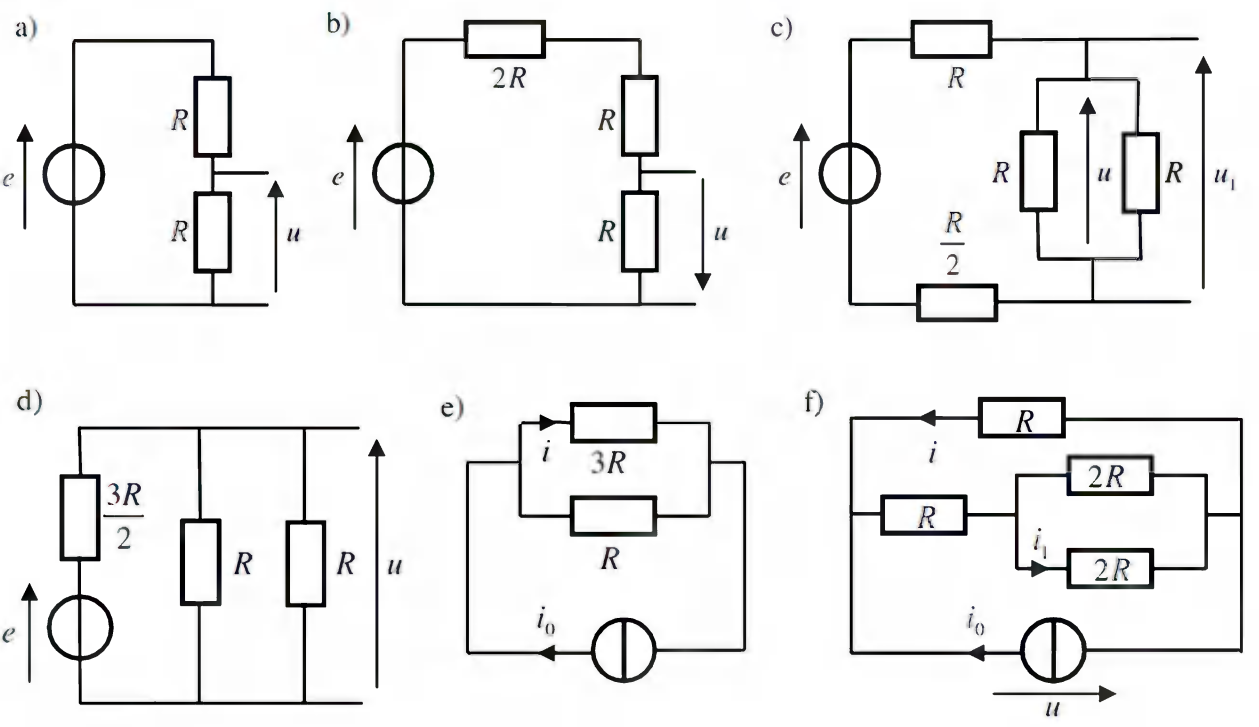
\includegraphics[width=\textwidth]{Images/exercicesKirchoff.png}

\subsection{Exercice 2}

\begin{minipage}[c]{\linewidth/2}
	\begin{circuitikz}
		%Circuit
		\draw (4, 0)
			to[short, i>=$I$] (2, 0)
			to[R, l=$R$] (0, 0)
			to[vsource, v_<=$e$] (0, -3)
			-- (4, -3);
		\draw (2, 0)
			to[R, l_=$R$, v^<=$U$] (2, -3);
	\end{circuitikz}
\end{minipage}%
\begin{minipage}[c]{\linewidth/2}
	On donne $R = \SI{10}{k\Omega}$.
	\begin{enumerate}
		\item Tracer la caractéristique du dipôle ci-contre.
		\item On ajoute une charge de résistance $R'=\SI{3}{k\Omega}$. Déterminer le point de fonctionnement de deux façons.
	\end{enumerate}
\end{minipage}

\subsection{Exercice 3 : Rendement d'un montage potentiométrique}

\begin{minipage}[c]{\linewidth/2}
	\begin{circuitikz}
		%Circuit
		\draw (0, 2)
		to[short, i>=$I$] (0, 3)
		--++(2, 0)
		to[R, l=$r_2$] ++(0, -2)
		to[R, l=$r_1$] ++(0, -2)
		--++(-2, 0)
		--++(0, 1)
		to[vsource, v=$E$] (0, 2);
		\draw (2, 1)
		to[short, i=$i_R$] ++(2, 0)
		to[R, l=$R$] ++(0, -2)
		--++(-2, 0);
	\end{circuitikz}
\end{minipage}%
\begin{minipage}[c]{\linewidth/2}
	Le rendement $\eta$ de ce diviseur de tension est le rapport $P_R$ de la puissance dissipée dans la résistance de charge $R$ à la puissance $P_E$ fournie par la source de tension $E$. Exprimer $\eta$ en fonction de $r_1$, $r_2$ et $R$.
	
	AN : $r_1 = \SI{750}{\Omega}$, $r_2=\SI{250}{\Omega}$, $R = \SI{80}{\Omega}$. Commentaire.
\end{minipage}

\subsection{Exercice 4 : Adaptation de puissance}

\begin{minipage}[c]{\linewidth/2}
	\begin{circuitikz}
		%Circuit
		\draw (0, 0)
		to[R, l=$R_0$] (3, 0)
		to[R, l=$R$] (3, -3)
		-- (0, -3)
		to[vsource, v=$E$] (0, 0);
	\end{circuitikz}
\end{minipage}%
\begin{minipage}[c]{\linewidth/2}
	Un générateur présente une tension à vide $E$ et une résistance interne $R_0$. On y branche une charge de résistance $R$. Pour quelle valeur de $R$ la puissance dissipée dans la résistance $R$ est elle maximale ? Que vaut alors cette puissance ?
\end{minipage}

\section{Semaine 02 (23/09-27/09) }


\e{Notions abordées :}
\begin{itemize}
	\item Circuits linéaires du premier ordre.
\end{itemize}

\subsection{Questions de cours}
\begin{enumerate}
	\item Relation entre la charge d'un condensateur et sa tension aux bornes.
	\item Relations entre intensité et tension pour un condensateur et une bobine.
	\item Continuité des grandeurs dans un circuit électrique.
	\item Établir l'expression de l'énergie stockée dans un condensateur/une bobine.
\end{enumerate}

\subsection{Exercice 1 : Résistance de fuite d'un condensateur}

Un condensateur réel présente des fuites de courants. Comment le modéliser ?

Il est inséré dans un circuit série comportant un générateur de f.é.m $E$, une résistance $r$ et un interrupteur $K$. On mesure la tension aux bornes du condensateur à l'aide d'un voltmètre idéal. On ferme $K$ et on attend que l'indication du voltmètre se stabilise. Puis on ouvre K en déclenchant au même instant un chronomètre. On constate que la tension indiquée par le voltmètre baisse de $10\%$ en un temps $T$.

On donne $E = \SI{1}{V}$, $r=\SI{10}{k\Omega}$, $T=\SI{1.0}{s}$ et $C=\SI{19}{\mu F}$.

\begin{enumerate}
	\item Exprimer la valeur $U$ vers laquelle la tension aux bornes du condensateur tend lorsque $K$ est fermé. En déduire une manière de déterminer $R_f$ (résistance de fuite).
	\item Montrer que la mesure du temps $T$ permet aussi de déterminer $R_f$. Commenter en relation avec l'une des hypothèses de l'énoncé.
\end{enumerate}

\subsection{Exercice 2 : Étude d'un circuit RL}

\begin{minipage}[c]{\linewidth/2}
	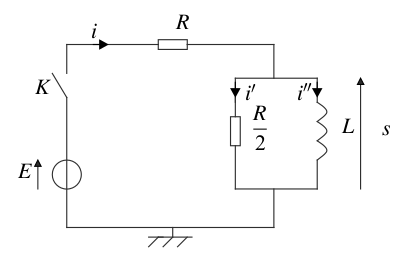
\includegraphics[width=\linewidth]{Images/mpsi_s02_ex02.png}
\end{minipage}%
\begin{minipage}[c]{\linewidth/2}
	À $t=0^-$, on ferme l'interrupteur $K$.
	\begin{enumerate}
		\item Donner $i$, $i'$, $i''$ et $s$ en $t=0^+$.
		\item Que vaut $s(t)$ lorsque $t$ tend vers l'infini.
		\item Établir l'équation différentielle vérifiée par $s(t)$.
		\item En déduire $s(t)$. En tracer l'allure.
		\item Exprimer le temps $t_0$ au bout duquel $s(t)$ a été divisé par $10$.
		\item On mesure $t_0=\SI{30}{\mu s}$ pour $R=\SI{1.0}{k\Omega}$. En déduire $L$.
	\end{enumerate}
\end{minipage}

\subsection{Exercice 3 : Rendement énergétique de la charge d'un condensateur}

On considère un circuit composé d'une résistance $R$ et d'un condensateur de capacité $C$ en série aux bornes duquel on place un générateur de tension idéal de f.é.m $E$ et un interrupteur $K$. À l'instant $t=0$, on ferme l'interrupteur $K$ et la tension $u_c$ aux bornes du condensateur est nulle.

\begin{enumerate}
	\item Établir l'équation différentielle vérifiée par $u_c$.
	\item Déterminer $u_c(t)$ et en tracer l'allure.
	\item Mêmes questions pour l'intensité du courant parcourant le circuit.
	\item Exprimer en fonction de $C$ et $E$ :
	\begin{itemize}
		\item L'énergie $\mathcal{E}_{elec}$ emmagasinée par le condensateur quand $t\rightarrow+\infty$.
		\item L'énergie $W_{Joule}$ dissipée par effet Joule dans la résistance entre $t=0$ et $t\rightarrow+\infty$.
		\item L'énergie $W_{gen}$ fournie par le générateur entre $t=0$ et $t\rightarrow+\infty$.
	\end{itemize}
	\item Donner une relation liant $\mathcal{E}_{elec}$, $W_{Joule}$ et $W_{gen}$ et proposer une interprétation physique de cette relation. Comment définir puis exprimer un rendement ?

\end{enumerate}
\section{Semaine 03 (30/09-04/10) }


\e{Notions abordées :}
\begin{itemize}
	\item Circuits linéaires du premier ordre (cf semaine précédente).
	\item Équilibre chimique.
\end{itemize}

\subsection{Questions de cours}
\begin{enumerate}
	\item Une mole de méthane réagit avec une mole de dioxygène selon une réaction de combustion. Déterminer la composition finale du système. (Équilibrer + Tableau d'avancement + Avancement final pour une réaction totale).
	\item Exprimer l'activité d'une espèce chimique dans un mélange. Préciser les hypothèses nécessaires.
	\item Exprimer le quotient réactionnel d'une réaction donnée et prévoir le sens d'évolution spontanée d'un système chimique.
\end{enumerate}

\subsection{Exercice 1 : Fluoration du dioxyde d'uranium}

Le dioxyde d'uranium solide réagit avec le fluorure d'hydrogène gazeux pour former du tétrafluorure d'uranium solide et de la vapeur d'eau. 

On maintient la température égale à $\SI{700}{K}$ et la pression totale à $\SI{1}{bar}$. La constante d'équilibre à $\SI{700}{K}$ est égale à $K^\circ = 6.8\times10^4$.

\begin{enumerate}
	\item Écrire la réaction.
	\item On part de $\SI{1.0}{mol}$ de dioxyde d'uranium et de $\SI{1.0}{mol}$ de fluorure d'hydrogène. Quelle sera la composition finale du système ?
	\item Même question en partant de $\SI{0.10}{mol}$ de dioxyde d'uranium et de $\SI{1.0}{mol}$ de fluorure d'hydrogène. Que remarque-t-on dans ce cas ?  
\end{enumerate}

\e{Réponses :}
\begin{enumerate}
	\item -
	\item $\xi = \SI{0.24}{mol}$.
	\item - 
\end{enumerate}

\subsection{Exercice 2 : Constante d'équilibre et quotient de réaction.}

Pour préparer industriellement du dihydrogène, on fait réagir en phase gazeuse du méthane avec de l'eau. La réaction produit également du monoxyde de carbone.

La réaction se déroule sous une pression totale constante $p_{tot} = \SI{10}{bar}$. La constante d'équilibre vaut $K^\circ = 15$. Initialement, le système contient $\SI{10}{mol}$ de méthane, $\SI{30}{mol}$ d'eau, $\SI{5}{mol}$ de monoxyde de carbone et $\SI{15}{mol}$ de dihydrogène. 

\begin{enumerate}
	\item Exprimer la constante d'équilibre en fonction des pressions partielles des constituants.
	\item Exprimer le quotient de réaction $Q$ en fonction de la quantité de matière de chacun des constituants et de la pression totale. Calculer $Q$ dans l'état initial.
	\item Le système est-il à l'équilibre thermodynamique ? Si non, dans quel sens se produira l'évolution ?
	\item Déterminer la composition du système à l'équilibre.
\end{enumerate}

\e{Réponses :}
\begin{enumerate}
	\item -
	\item $Q = 1.56$.
	\item -
	\item $\xi = \SI{3.6}{mol}$.
\end{enumerate}

\subsection{Exercice 3 : Utilisation du quotient de réaction.}

Un récipient de volume $V_0 = \SI{2.00}{L}$ contient initialement $\SI{0.500}{mol}$ de COBr$_2$ qui se décompose à une température de $\SI{346}{K}$ selon la réaction : $$\ce{COBr2_{(g)} = CO_{(g)} + Br2_{(g)}}$$.

\begin{enumerate}
	\item Déterminer la composition du système à l'équilibre sachant que la constante d'équilibre à $\SI{346}{K}$ vaut $K^\circ = 5.46$.
	\item Calculer le pourcentage de COBr$_2$ décomposé à cette température.
	\item L'équilibre précédent étant réalisé, on ajoute $\SI{2.00}{mol}$ de monoxyde de carbone. L'équilibre chimique est-il réalisé ? Si non, décrire l'évolution ultérieure du système.
\end{enumerate}

\e{Réponses :}
\begin{enumerate}
	\item $\xi = \SI{0.285}{mol}$.
	\item 57 \%.
	\item $Q = 43.2$, $\xi' = \SI{0.077}{mol}$.
\end{enumerate}
\section{Semaine 04 (07/10-11/10) }


\e{Notions abordées :}
\begin{itemize}
	\item Équilibre chimique (cf semaine précédente).
	\item Bases de l'optique géométrique.
\end{itemize}

\subsection{Questions de cours}
\begin{enumerate}
	\item Énoncer les lois de Snell-Descartes.
	\item Définir un rayon lumineux et un MTHI.
	\item Indice de réfraction ? Phénomène de réflexion totale ?
\end{enumerate}

\subsection{Exercice 1 : Réfractomètre de Pulrich}

\begin{minipage}[c]{\linewidth/2}
	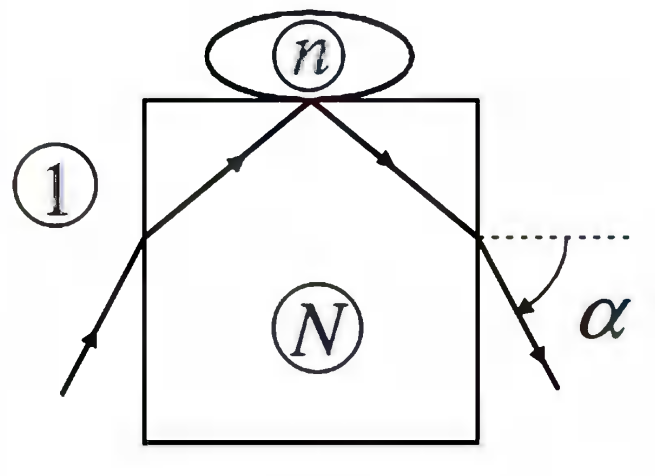
\includegraphics[width=\linewidth]{Images/mpsi_s04_ex01.png}
\end{minipage}%
\begin{minipage}[c]{\linewidth/2}
	Un réfractomètre de Pulrich est constitué d'un cube de verre d'indice $N$ connu sur lequel on a déposé une goutte d'un liquide d'indice $n$ inconnu. On observe un faisceau de rayons parallèles à la limite réfraction - réflexion totale et on mesure l'angle $\alpha$ correspondant. On donne $N=1.626$ et $\alpha=60$°.
\end{minipage} 

\begin{enumerate}
	\item Que vaut $n$ ?
	\item Quelles sont les valeurs mesurables de $n$ avec ce dispositif ?
\end{enumerate}

\e{Réponse} : $n = 1.376$

\subsection{Exercice 2}

\begin{minipage}[c]{\linewidth/2}
	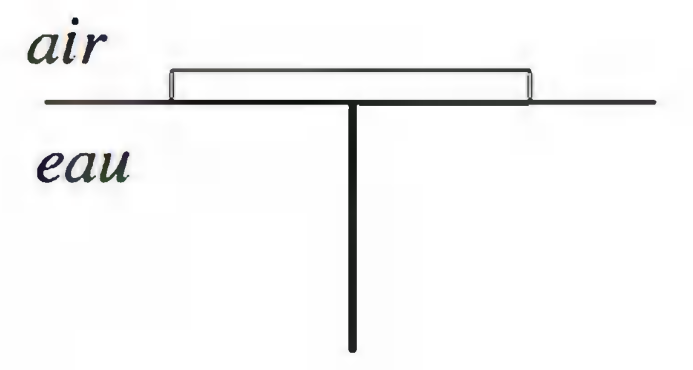
\includegraphics[width=\linewidth]{Images/mpsi_s04_ex02.png}
\end{minipage}%
\begin{minipage}[c]{\linewidth/2}
	Un disque en liège de diamètre $D = \SI{5}{cm}$ flotte sur l'eau. Il soutient une tige placée perpendiculairement en son centre. 
	
	Quelle est la longueur $h$ de la partie de la tige qu'un observateur dans l'air ne peut pas voir ?
\end{minipage}

\e{Réponse :} $h = \SI{2.1}{cm}$.

\subsection{Exercice 3 : Détection de pluie sur un pare-brise}

\begin{minipage}[c]{\linewidth/2}
	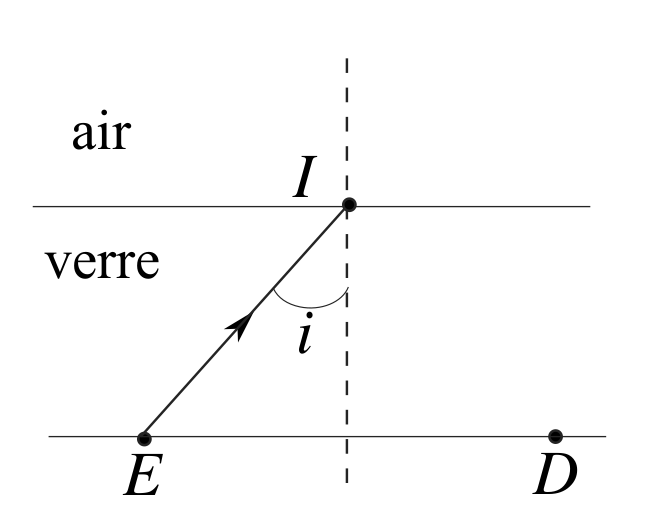
\includegraphics[width=\linewidth]{Images/mpsi_s04_ex03.png}
\end{minipage}%
\begin{minipage}[c]{\linewidth/2}
	On modélise un pare-brise par une lame de verre à faces parallèles, d'épaisseur $e = \SI{5}{mm}$, d'indice $n_v = 1.5$. Un fin pinceau lumineux issu d'un émetteur situé en $E$ arrive de l'intérieur du verre sur le dioptre verre/air en $I$ avec un angle d'incidence $i=60$°.
\end{minipage}

\begin{enumerate}
	\item Montrer que le flux lumineux revient intégralement sur le détecteur situé en $D$ et déterminer la distance $ED$.
	\item Comment ce dispositif permet-il de détecter un dépôt de pluie sur le pare-brise ? On supposera une épaisseur d'eau de $\SI{1}{mm}$.
\end{enumerate}

\e{Réponses :}
\begin{enumerate}
	\item $i_{lim} = 41.8$°.
	\item Distance au détecteur de $\SI{0.9}{cm}$.
\end{enumerate}


\section{Semaine 05 (14/10-18/10) }


\e{Notions abordées :}
\begin{itemize}
	\item Bases de l'optique géométrique (cf semaine précédente).
	\item Systèmes optiques.
\end{itemize}

\subsection{Questions de cours}

\textit{Cf exercices}

\subsection{Exercice 1 : Méthode de Bessel pour la focométrie}

On considère un objet transverse (AB) et un écran distants de $D$, ainsi qu'une lentille convergente de focale $f'$.

\begin{enumerate}
	\item Tracer les rayons dans le cas d'une image réelle.
	\item À quelle condition peut-on former l'image de l'objet sur l'écran ? Démonstration.
	\item Déterminer les positions de la lentille qui permettent d'obtenir une image sur l'écran. En déduire une méthode pour déterminer $f'$.
\end{enumerate}

\subsection{Exercice 2 : Microscope}

\begin{minipage}[c]{\linewidth/2}
	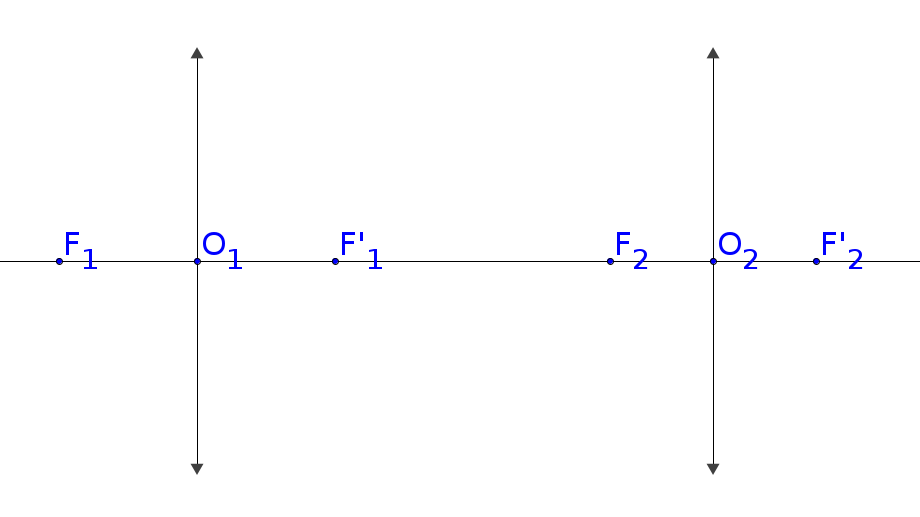
\includegraphics[width=\textwidth]{./Images/mpsi_s05_ex02.png}
\end{minipage}%
\begin{minipage}[c]{\linewidth/2}
	On donne $\overline{O_1O_2} = D_0 = \SI{75}{mm}$, $f'_1 = \SI{10}{mm}$ et $f'_2 = \SI{25}{mm}$.
\end{minipage}
 
\begin{enumerate}
	\item Que sont les conditions de Gauss et à quoi servent elles ?
	\item On pose $\Delta = \overline{F'_1F'_2}$. Exprimer $\Delta$ en fonction des données du problème. Calcul.
	\item On souhaite qu'un œil au repos voie l'image $A'B'$ de $AB$ par le système optique. Où est $A'B'$.
	\item Où doit alors être l'image intermédiaire $A_1B_1$ ?
	\item Exprimer la position de l'objet $AB$ en fonction de $f'_1$ et $\Delta$. Calcul.
	\item Étude du grossissement :
	\begin{enumerate}
		\item Quelle est la taille maximale de l'image que l'on peut avoir sur la rétine sans microscope ?
		\item Quelle est la taille de l'image sur la rétine avec microscope ?
		\item En déduire le "grossissement commercial" du microscope.
	\end{enumerate}
\end{enumerate}

\subsection{Exercice 3 : Lunette astronomique}

On souhaite observer Mars. Soit $\alpha$ le diamètre angulaire sous lequel elle est vue à l'œil nu. Pour cela on utilise un système optique composé de deux lentilles convergentes de focales respectives $f'_1=f'_{obj}$ et $f'_2=f'_{oc}$ (l'oculaire est du côté de l'œil, l'objectif est du côté de l'objet Mars).

\begin{enumerate}
	\item On utilise un système afocal. Définir afocal. En déduire la position relative des deux lentilles.
	\item Faire le tracé des rayons. L'image est-elle droite ou renversée ?
	\item Soit $\alpha'$ le diamètre angulaire en sortie du système optique. Exprimer le grossissement $G = \alpha'/\alpha$. Interpréter cette grandeur.
	\item \label{qprec} On veut augmenter le grossissement et renverser l'image. On interpose entre l'objectif et l'oculaire une troisième lentille convergente de focale $f'_3$. On déplace l'oculaire pour pouvoir observer l'image au repos. Quel couple de points cette nouvelle lentille doit elle conjuguer ?
	\item Faire le tracé des rayons.
	\item Soit $\gamma_3$ le grandissement de la nouvelle lentille associé au couple de points de la question \ref{qprec}. Exprimer $\overline{O_3F'_{obj}}$ en fonction de $\gamma_3$ et $f'_3$.
	\item Quel est le grossissement $G'$ de ce nouveau système optique. Le comparer à $G$ et conclure.
\end{enumerate}


\subsection{Exercice 4 : Stigmatisme d'une lame à faces parallèles}

Une lame à faces parallèles d'épaisseur $e$ est constituée d'un verre d'indice $n$. Elle est placée dans l'air. 

\begin{enumerate}
	\item Construire le cheminement d'un rayon arrivant sur le premier dioptre avec l'incidence $i$. Soit $r$ l'angle de réfraction. Le rayon transmis par la lame est-il dévié par rapport au rayon incident ? Comment appeler la modification subie ?
	\item On considère un objet ponctuel $A$ sur le rayon incident. Calculer la distance entre le prolongement du rayon incident et le rayon transmis en fonction de $e$, $i$ et $r$. 
	\item Rappeler ce qu'est le stigmatisme. Le système considéré est-il stigmatique ?
	\item On se place maintenant dans les conditions de Gauss. Montrer que le système est approximativement stigmatique et déterminer la relation de conjugaison donnant $\overline{AA'}$ en fonction de $n$ et $e$.
	\item Dans un parc aquatique, les aquariums ont une épaisseur de verre de $\SI{60}{cm}$. Situé à $\SI{20}{cm}$ de la vitre, un visiteur observe un requin marteau nageant à $\SI{1.0}{m}$ devant lui. À quelle distance semble-t-il être pour l'observateur ?
\end{enumerate}

\e{Réponse :} $\overline{R'A} = \SI{75.0}{cm}$.

\section{Semaine 06 (04/11-08/11) }


\e{Notions abordées :}
\begin{itemize}
	\item Systèmes optiques (cf semaine précédente).
	\item Cinétique chimique.
\end{itemize}

\subsection{Questions de cours}

\begin{enumerate}
	\item Définir la vitesse d'une réaction chimique. Quelle est son unité ?
	\item Qu'est ce que l'ordre d'une réaction chimique ? L'ordre partiel ? La constante de vitesse ?
	\item Donner la loi d'Arrhenius.
\end{enumerate}

\subsection{Exercice 1 : Décomposition de l'azométhane en phase gazeuse}

Dans un récipient de volume fixé $V$, on introduit à $\SI{600}{K}$ de l'azométhane \ce{CH3N2CH3_{(g)}}. Celui-ci se décompose en éthane et en diazote gazeux. 

L'évolution de la réaction est suivie par manométrie et une série de mesures a donné la pression partielle $p_A$ en azométhane : 

\begin{tabular}{|c|c|c|c|c|c|}
	\hline 
	$t$ ($10^3$ s) & $0$ & $1.00$ & $2.00$ & $3.00$ & $4.00$ \\ \hline
	$p_A$ ($10^{-2}$ mmHg) & $p_0 = 8.21$ & $5.74$ & $4.00$ & $2.80$ & $1.96$ \\ \hline
\end{tabular}

\begin{enumerate}
	\item Écrire l'équation bilan de la réaction.
	\item Vérifier que la réaction est d'ordre $1$ par rapport au réactif et calculer sa constante de vitesse.
\end{enumerate}

\e{Réponse :} $k = \SI{3.58e-4}{\per\second}$

\subsection{Exercice 2 : Temps de demi-réaction}

La réaction de décomposition totale du pentaoxyde de diazote \ce{N2O5} en dioxyde d'azote \ce{NO2} et dioxygène a lieu en phase gazeuse. L’expérience est menée dans un récipient de volume V constant, initialement vide, en amenant du pentaoxyde de diazote de manière à ce que la pression initiale soit $p_0$.

\begin{enumerate}
	\item On mesure la pression $p(t)$ au cours du temps. On veut évaluer la constante cinétique en mesurant le temps de demi-réaction. Quelle doit être la lecture de $p$ sur le manomètre pour ce temps ?
	\item Le tracé de la courbe $\ln{p(\ce{N2O5})}$ en fonction du temps est une droite. En déduire l'ordre de la réaction. Tracer l'allure de la pression en fonction du temps.
	\item Une première mesure réalisée à $\theta = \SI{150}{\celsius}$ permet de mesurer un temps de demi réaction $t_{1/2} = \SI{7.5}{s}$. Une seconde mesure réalisée à $\theta' = \SI{100}{\celsius}$ permet de mesurer un temps de demi-réaction $t'_{1/2} = \SI{7.0}{min}$. Calculer la constante de vitesse pour ces deux températures.
	\item Calculer l'énergie d'activation de la réaction.
\end{enumerate}

\e{Réponses :}
\begin{enumerate}
	\item $p_{1/2} = \frac{7}{4}p_0$.
	\item -
	\item $k = \SI{9.2e-2}{\per\second}$ et $k' = \SI{1.7e-3}{\per\second}$.
	\item $E_a = \SI{1.1e2}{\kilo\joule\per\mol}$.
\end{enumerate}

\subsection{Exercice 3 : Dismutation des ions hypochlorites}

En solution aqueuse, les ions hypochlorite \ce{ClO-} peuvent se dismuter selon la réaction totale $$\ce{ClO- = \frac{1}{3} ClO3- + \frac{2}{3}Cl-}$$.

La vitesse de la réaction $r$, définie comme la vitesse de disparition des ions hypochlorite \ce{ClO-} suit une loi cinétique de second ordre, dont la constante de vitesse est notée $k$.

On provoque cette réaction dans une solution contenant initialement des ions hypochlorite à la concentration $c_0 = \SI{0.10}{\mol\per\liter}$.

À $T = \SI{343}{K}$, la constante de vitesse de la solution est $k = \SI{3.1e-3}{\per\mol \deci \meter \cubed \per \second}$. 

L’énergie d’activation de cette réaction au voisinage des températures considérées ici est $E_a = \SI{47}{\kilo\joule\per\mol}$.

\begin{enumerate}
	\item Donner l’équation horaire de la concentration en ions hypochlorite.
	\item Au bout de combien de temps, noté $t_{30}$, aura-t-on obtenu la disparition de $30\%$ des ions hypochlorite ?
	\item Quel serait à $T' = \SI{363}{K}$ le temps $t_{30}'$ nécessaire pour obtenir le même taux d'avancement de $30 \%$ à partir de la même solution initiale ?
\end{enumerate}

\e{Réponses :}
\begin{enumerate}
	\item -
	\item $t_{30} = \SI{23}{min}$.
	\item $t_{30}' = \SI{9}{min}~\SI{20}{s}$.
\end{enumerate}


\section{Semaine 07 (11/11-15/11) }


\e{Notions abordées :}
\begin{itemize}
	\item Cinétique chimique (cf semaine précédente).
	\item Oscillateurs harmoniques.
\end{itemize}

\subsection{Questions de cours}

\begin{enumerate}
	\item Établir et reconnaître l'équation d'un circuit $LC$. La résoudre compte tenu des conditions initiales.
	\item Résoudre l'équation de l'oscillateur harmonique avec les conditions initiales $u(0)=3E$ et $\dot{u}(0)=4 \omega E$. Quelle est la phase à l'origine ?
	\item Dans le cadre du circuit $LC$ libre montrer la conservation et l'équipartition de l'énergie (conditions initiales arbitraires).
\end{enumerate}

\e{Exercices de chimie cf semaine précédente.}


\section{Semaine 08 (18/11-22/11) }


\e{Notions abordées :}
\begin{itemize}
	\item Oscillateur harmonique (cf semaine précédente).
	\item Oscillateur amorti.
\end{itemize}

\subsection{Questions de cours}

\begin{enumerate}
	\item Établir l'équation d'un circuit $RLC$ série.
	\item Donner l'équation de l'oscillateur amorti et ses solutions dans le cas général.
	\item Résoudre l'équation de l'oscillateur harmonique avec les conditions initiales $u(0)=3E$ et $\dot{u}(0)=4 \omega E$. Quelle est la phase à l'origine ?
\end{enumerate}

\subsection{Exercice 1 : Exemple de régime critique}

\begin{minipage}[c]{\linewidth/2}
	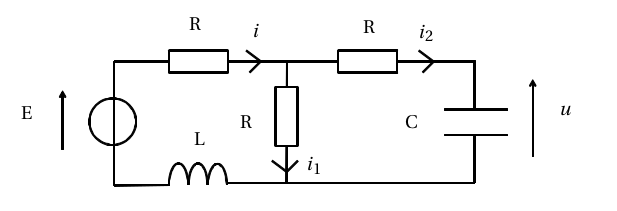
\includegraphics[width=\textwidth]{/home/chams/Documents/Travail/2024-2025/Colles/Images/mpsi_s08_ex01.png}
\end{minipage}%
\begin{minipage}[c]{\linewidth/2}
	Initialement le condensateur est déchargé et aucun courant ne traverse la bobine.
\end{minipage}

\begin{enumerate}
	\item Déterminer l'équation différentielle vérifiée par $u(t)$.
	\item Quelle est la relation entre $R$, $L$ et $C$ pour vérifier la condition de régime critique ? On suppose cette condition vérifiée dans la suite.
	\item Quelles sont les conditions initiales ? Déterminer également $u(\infty)$ et $i(\infty)$.
	\item Déterminer $u(t)$.
\end{enumerate}

\e{Réponses :}
\begin{enumerate}
	\item $u'' + 1/2(3R/L + 1/RC)u' + u/LC = E/2LC$
	\item $L = R^2 C$
	\item $u=0$, $u'=0$.
	\item $u(t) = E/2 - E/2(1+t/RC)e^{-t/RC}$
\end{enumerate}

\subsection{Exercice 2 : Étude d'un circuit à deux bobines}

\begin{minipage}[c]{\linewidth/2}
	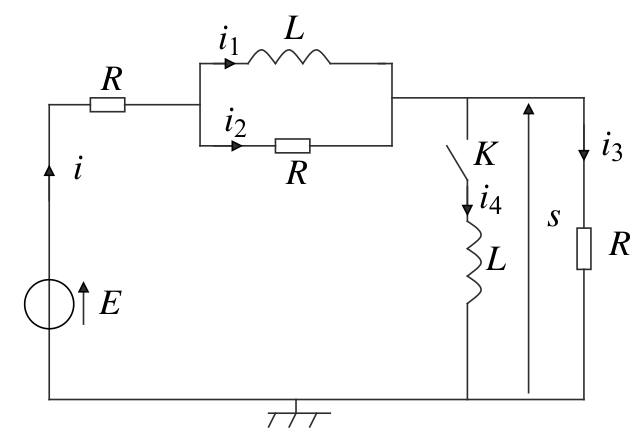
\includegraphics[width=\textwidth]{/home/chams/Documents/Travail/2024-2025/Colles/Images/mpsi_s08_ex02.png}
\end{minipage}%
\begin{minipage}[c]{\linewidth/2}
	À $t=0$, on ferme $K$
\end{minipage}

\begin{enumerate}
	\item Établir l'équation différentielle vérifiée par $s(t)$.
	\item Déterminer les conditions initiales pour $i$, $i_1$, $i_2$, $i_3$ et $i_4$. Déterminer également leurs valeurs pour $t\rightarrow+\infty$.
	\item Déterminer $s(t)$. 
\end{enumerate}

\e{Réponses :}
\begin{enumerate}
	\item $3s'' + 4R/L s' + (R/L)^2 s = 0$
	\item En $t=0^+$, $i_1=E/2R$, $i_3=E/2R$, $i=E/R$, $i_2=0$, $i_4=0$.
	\item $s(t) = \frac{E}{4} \left( \exp -\frac{R}{L}t +  \exp -\frac{R}{3L}t \right)$
\end{enumerate}


\subsection{Exercice 3 : Réponse à un échelon de tension d'un dipôle $RLC$ parallèle}

\begin{minipage}[c]{\linewidth/2}
	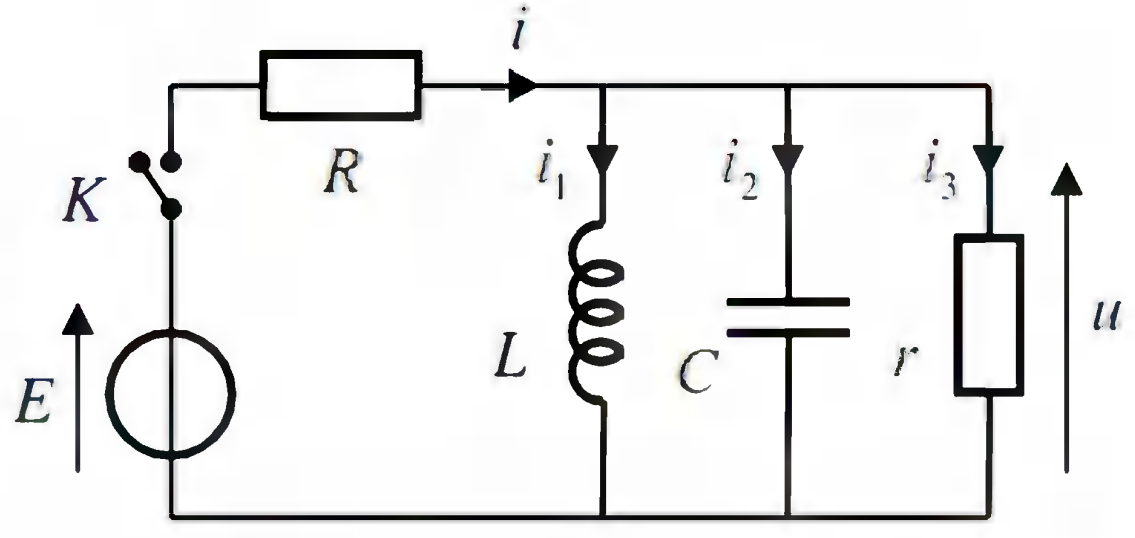
\includegraphics[width=\textwidth]{/home/chams/Documents/Travail/2024-2025/Colles/Images/mpsi_s08_ex03.png}
\end{minipage}%
\begin{minipage}[c]{\linewidth/2}
	Pour $t<0$, le condensateur est déchargé et la bobine idéale n'est parcourue par aucun courant. À $t=0$, on ferme $K$
\end{minipage}

\begin{enumerate}
	\item Établir l'équation différentielle vérifiée par $i_3$. La mettre sous forme canonique.
	\item Déterminer les conditions initiales. Déterminer également la valeur de $i_3$ pour $t\rightarrow+\infty$.
	\item Donner la relation entre $R$, $r$, $L$ et $C$ pour que le régime soit de type pseudopériodique et exprimer $i_3(t)$ dans ce cas.
\end{enumerate}

\e{Réponses :}
\begin{enumerate}
	\item $\omega_0 = \frac{1}{\sqrt{LC}}$, $\frac{\omega_0}{Q} = \frac{R + r}{RrC}$.
	\item En $t=0^+$, $u=0$, $i_1=0$, $i_3=0$, $i=E/R$, $i_2=E/R$. En $t\rightarrow+\infty$, $u=0$, $i=i_1=E/R$, $i_2=i_3=0$
	\item $\frac{2rR}{R+r} > \sqrt{\frac{L}{C}}$
\end{enumerate}


\section{Semaine 09 (25/11-29/11) }


\e{Notions abordées :}
\begin{itemize}
	\item Oscillateurs.
	\item Propagation d'un signal
\end{itemize}

\subsection{Questions de cours}

\begin{enumerate}
	\item Citer quelques exemples d'ondes. Préciser leurs caractéristiques (polarisation, milieu de propagation, ordre de grandeur de la célérité).
	\item Qu'est-ce qu'une onde progressive ?
	\item Qu'est ce qu'une onde progressive sinusoïdale ?
\end{enumerate}

\e{Exercices : cf semaine précédente}

\section{Semaine 10 (02/12-06/12) }


\e{Notions abordées :}
\begin{itemize}
	\item Propagation d'un signal (cf. semaine précédente).
	\item Phénomènes ondulatoires.
\end{itemize}

\subsection{Questions de cours}

\begin{enumerate}
	\item Relation donnant la demi-largeur angulaire de la tâche centrale de diffraction par une fente de largeur $a$, avec une lumière de longueur d’onde $\lambda$.
	\item Conditions d'interférences constructives et destructives en fonction du déphasage, puis de la différence de marche.
	\item Lien entre l'intensité lumineuse et le signal lumineux. Cas d'un signal sinusoïdal. Pourquoi un capteur lumineux n'est il sensible qu'à l'intensité lumineuse ?
\end{enumerate}

\subsection{Exercice 1 : Interférences acoustiques}

Deux haut-parleurs $S_1$ et $S_2$ alimentés par le même signal $s(t) = s_0 cos (\omega t)$ de fré-
quence $f = \SI{2,0}{kHz}$ sont disposés face à face en $x = 0$ et $x = L$. On place un microphone au point $M$ d’abscisse $x_M$ qui capte l’onde résultant de la superposition des ondes issues des deux émetteurs sachant que les ondes sonores issus de chaque haut parleur se propage à vitesse c et ont une longueur d’onde $\lambda$. En déplaçant le microphone, on repère des zones de l’espace où l’amplitude du signal prend des valeurs maximales.

\begin{enumerate}
	\item Établir les expressions des signaux $s_1(t)$ et $s_2(t)$ correspondant aux ondes acoustiques émises par $S_1$ et $S_2$.
	\item En déduire le déphasage $\phi = \phi_2-\phi_1$ entre les deux ondes au point $M$ d'abscisse $x$ en fonction de $x$, $\lambda$ et $L$.
	\item En déduire les positions $x_c$ des points de l'espace où l'on observe des interférences constructives. Déterminer l'interfrange.
	\item Retrouver ces valeurs en ne raisonnant qu'en terme de trajet parcouru par les ondes.
	\item L'interfrange vaut $\SI{8,6}{cm}$. En déduire la vitesse du son $c$.
\end{enumerate}

\subsection{Exercice 2 : Corde de Melde}

On considère une corde de longueur $L$, fixée en $O$ à gauche et libre d'osciller en $M$ à droite.

\begin{enumerate}
	\item Un opérateur fait osciller l'extrêmité $M$ de la corde verticalement, entre $-z_0$ et $+z_0$ à la pulsation $\omega$. Écrire l'onde progressive qui se propage vers la gauche la vitesse $c$.
	\item On rappelle que la corde est fixée en $O$. Justifier qu'il existe une onde réfléchie et l'écrire.
	\item Calculer l'onde totale. Comment appelle-t-on une telle onde ?
	\item On rappelle que le mouvement est forcé au point $M$. En déduire les pulsations possibles d'oscillation. Commenter.
\end{enumerate}

\subsection{Exercice 3 : La couleur bleue du papillon Morpho}

Une source monochromatique ponctuelle $S$, située dans l'air, de longueur d'onde $\lambda$ éclaire une couche transparente d'indice $n$ et d'épaisseur $e$ en $I$ avec l'angle d'incidence $i$. Un rayon noté $(1)$ est alors réfléchi dans l'air d'indice $n_0$ et un autre rayon $(2)$ est réfracté avec un angle $r$ puis réfléchi en bas de la couche au point $J$, avant d'être réfracté au point $K$ avec un angle $i'$ dans l'air.

Un observateur reçoit les deux rayons lumineux.

On admettra que la notion $(AB)$ désigne la distance $AB$ multipliée par l'indice du milieu dans lesquels sont $A$ et $B$ : $(AB) = n AB$.

\begin{enumerate}
	\item Expliquer pourquoi les rayons $(1)$ et $(2)$ ressortent parallèles. En déduire qu'ils interfèrent sur la rétine.
	\item La différence de marche est donnée par $\delta = (IJ)+(JK)-(IH) + \lambda/2$ où le dernier terme moins évident est lié à la réflexion en $J$. Exprimer $\delta$ en fonction de $e$, $n$, $n_0$, $i$ et $\lambda$.
	\item L'aile du papillon morpho est composé de petites lamelles de chitine d'indice $n=1,7$. On observe une couleur intense dans le bleu pour un angle de vue $i=\SI{30}{\degree}$. Si toutefois on plonge l'aile dans l'acétone d'indice $n_0=1,4$, la couleur est verte. Expliquer ces phénomènes. 
\end{enumerate}

\section{Semaine 11 (09/12-13/12) }


\e{Notions abordées :}
\begin{itemize}
	\item Phénomènes ondulatoires (cf. semaine précédente).
	\item Structure des entités chimiques.
\end{itemize}

\subsection{Questions de cours}

\begin{enumerate}
	\item Établir de façon détaillée la configuration électronique de l'atome d'azote dans son état fondamental.
	\item Établir de façon détaillée la représentation de Lewis de la molécule de dioxyde de carbone.
	\item Évolution des propriétés dans le tableau périodique (Masse atomique (déf ?), Électronégativité (déf ?), éventuellement rayon atomique.)
\end{enumerate}

\subsection{Exercice : Formules de Lewis}

\begin{enumerate}
	\item \ce{HNO2}, \ce{O3}, \ce{N3-}, \ce{SO2}, \ce{SO3}.
	\item \ce{LiH}, \ce{BeH2}, \ce{BBr3}, \ce{AlN}, \ce{AlCl3}.
\end{enumerate}
\section{Semaine 12 (16/12-20/12) }


\e{Notions abordées :}
\begin{itemize}
	\item Structure des entités chimiques (cf semaine précédente).
	\item Cinématique du point matériel.
\end{itemize}

\subsection{Questions de cours}

\begin{enumerate}
	\item Expression du vecteur position $\vec{OM}$ en coordonnées cartésiennes, polaires et cylindrique + dessin.
	\item Expression du vecteur déplacement infinitésimal $\vec{dOM}$ en coordonnées cartésiennes, polaires et cylindriques.
	\item Expression de l'accélération en coordonnées cartésiennes, polaires et cylindriques.
\end{enumerate}

\subsection{Exercice 1 : Fronde}

Un jeune garçon s’amuse à faire tourner un caillou accroché au bout d’une corde de longueur $R = \SI{1.2}{m}$ dans un plan horizontal à une hauteur $h=\SI{1.8}{m}$ au-dessus du sol selon un mouvement circulaire. La vitesse devenant trop grande, la corde se casse et le caillou part horizontalement pour tomber à une distance $d = \SI{9.1}{m}$ de son point de décrochage. Il est soumis durant cette phase à la seule accélération de pesanteur $g$ qu’on prendra égale en norme à $g = \SI{9.8}{\meter\per\second\squared}$. 

Quelle était l’accélération centripète radiale au moment de la rupture ? Commentaire.

\e{Réponse :} $\SI{190}{\meter\per\second\squared}$

\subsection{Exercice 2 : Balle lancée depuis une montgolfière}

Une montgolfière se déplace à l'altitude $h = \SI{100}{m}$ constante avec une vitesse horizon-
tale de 10 m.s−1 . Un passager lance une balle vers le haut suivant la verticale mais du
fait de l’entraînement horizontal dû au déplacement de la montgolfière, la vitesse ini-
tiale résultante de la balle est inclinée d’un angle α = 40◦ par rapport à l’horizontale
pour quelqu’un observant la chute depuis le sol. La balle subit alors une accélération
descendante constante g = 9,8 m.s−2 .
a) Quelle est la durée de la chute ?
b) Déterminer le lieu où la balle touche le sol.
c) Déterminer la vitesse avec laquelle la balle arrive au sol.
d) Comparer les déplacements horizontaux de la balle et de la montgolfière. En dé-
duire la nature de la trajectoire de la balle pour le passager de la montgolfière.

\subsection{Exercice 3 : Cycliste sur piste}

La piste d’un vélodrome est constituée de deux demi-cercles de rayon R = 23 m rac-
cordés par deux portions rectilignes de longueur ℓ = 53 m.
a) Calculer la longueur de la piste.
b) Un cycliste sur piste est-il en rotation ou en translation circulaire ?
c) Il atteint une vitesse de 51 km.h−1 sur la partie circulaire de rayon R = 10 m. Dé-
terminer sa vitesse angulaire.
d) Déterminer la fréquence du mouvement sachant que la longueur de la partie rec-
tiligne est ℓ = 68 m.

\section{Semaine 13 (06/01-10/01) }


\e{Notions abordées :}
\begin{itemize}
	\item Structure des entités chimiques (cf semaine précédente).
	\item Cinématique du point matériel (cf semaine précédente).
	\item Dynamique du point matériel.
\end{itemize}

\subsection{Questions de cours}

\begin{enumerate}
	\item Définir un référentiel. Définir un référentiel galiléen. Donner des exemples de référentiels galiléens ou non galiléens.
	\item Donner les trois lois de Newton.
	\item Déterminer l'équation différentielle des oscillations d'un pendule simple.
\end{enumerate}

\subsection{Exercice 1 : Descente et chute d'un skieur}

Un skieur descend une piste faisant un angle $\alpha$ avec l’horizontale. On suppose une force de frottement de l’air $\vec{F}$ de norme $\lambda ||\vec{v}||$. On note $\vec{T}$ et $\vec{N}$ les composantes de la réaction de la neige sur les skis et $f$ le coefficient de frottement. On rappelle que s'il y a glissement, on a $||\vec{T}|| = f ||\vec{N}||$.

\begin{enumerate}
	\item Exprimer $T$ et $N$ en fonction des paramètres du problème.
	\item Établir l’équation différentielle en $v(t)$, la vitesse du skieur.
	\item Montrer que le skieur atteint une vitesse limite $v_L$. L'exprimer en fonction de $m$, $\lambda$, $f$, $g$ et $\alpha$. A.N. $\lambda = \SI{1.0}{\newton \second \per \meter}$, $f = 0.9$, $g = \SI{10}{\meter\per\second\squared}$, $m = \SI{80}{kg}$ et $\alpha = \SI{45}{\degree}$.
	\item Calculer la vitesse $v(t)$ et la position $x(t)$ du skieur en fonction de $v_L$, $\lambda$ et $m$.
	\item Calculer l’instant où le skieur atteint une vitesse $v_L/2$.
	\item Il tombe et à partir de ce moment-là, on néglige la résistance de l’air mais le coefficient de frottement est multiplié par $10$. Déterminer la distance parcourue avant de s’arrêter.
\end{enumerate}

\e{Réponses :}
\begin{enumerate}
	\item -
	\item -
	\item $v_L = \SI{57}{\meter\per\second}$
	\item -
	\item $\SI{55}{s}$
	\item $\SI{7.3}{\meter}$
\end{enumerate}

\subsection{Exercice 2 : Un tour en traîneau}

Un traîneau tiré par des chiens se déplaçant sur un sol horizontal est assimilé à un point matériel de masse $M = \SI{5.0e2}{kg}$. La réaction du support est $\vec{R} = \vec{T}+\vec{N}$. $\vec{N}$ est la composante normale à la surface. $\vec{T}$ est la composante tangentielle. On rappelle que 
\begin{itemize}
	\item le traîneau est immobile tant que $||\vec{T}|| < \mu_s ||\vec{N}||$,
	\item s'il y a glissement, $||\vec{T}|| = \mu_d ||\vec{N}||$.
\end{itemize}
avec $\mu_d = \SI{5.0e-2}{}$  et $\mu_s = \SI{8.0e-2}{}$.

On note $\vec{F}$ la force de traction exercée par les chiens sur le traîneau et on admet $||\vec{F}|| = F = F_0 - \beta ||\vec{v}||$ avec $F_0, \beta > 0$.

\begin{enumerate}
	\item Exprimer la valeur minimale de $F_0$ qui permet le démarrage du traîneau. Application numérique. Commentaire.
	\item Le traîneau est en mouvement rectiligne. Déterminer l'équation différentielle sur la vitesse. On définira un temps caractéristique $\tau$.
	\item Exprimer la vitesse limite $v_L$ atteinte par le traîneau en fonction des paramètres du problème.
	\item Déterminer $v(t)$. Tracer son allure. Faire figurer le temps $\tau$.
	\item $v_L$ est atteinte à $5\%$ près au bout d'un temps $t_1 = \SI{5.0}{s}$. Exprimer $\beta$ en fonction de $M$ et $t_1$. Application numérique.
	\item On donne $v_L = \SI{3.0}{\meter\per\second}$. En déduire $F_0$. Commentaire.
	\item Désormais à vitesse constante $v_L$, le traîneau aborde une courbe assimilée à un virage circulaire de rayon $R$ et de centre $O$. Soit $\alpha$ l'angle entre $\vec{F}$ et $\vec{v}$ Déterminer la norme $F$ de la force exercée par les chiens, ainsi que $\tan{\alpha}$ en fonction de $v_L$, $R$, $\mu_d$, $g$ et $M$, afin de maintenir cette trajectoire circulaire.
\end{enumerate}

\e{Réponses :}
\begin{enumerate}
	\item $F_{0, min} = \SI{392}{N}$
	\item -
	\item -
	\item -
	\item $\beta = \SI{300}{kg\per\second}$
	\item $F_0 = \SI{1.1e3}{N}$
	\item $\tan\alpha = \frac{v_L^2}{R \mu_d g}$ et $F = M\sqrt{ \left(\frac{v_L^2}{R}\right)^2 + (\mu_d g)^2}$
\end{enumerate}

\subsection{Exercice 3 : Oscillations amorties d'un plateau}

Une boule de pâte à modeler de masse $m = \SI{250}{g}$ tombe en chute libre d'une hauteur $h_0 = \SI{40}{cm}$ sur un plateau immobile, de masse négligeable et supporté par un ressort vertical. On considère qu'au moment du contact il n'y a pas de perte d'énergie cinétique, c'est-à-dire que la boule à la même vitesse juste avant le contact, et juste après lorsqu'elle est solidaire du plateau et se met à osciller avec lui.

L'origine des altitudes est prise à la position initiale du plateau.

\begin{enumerate}
	\item Sachant que le ressort a pour raideur $k = \SI{500}{N\per\meter}$, déterminer la hauteur $h_1$ dont s'affaisse le plateau. Quelle est la hauteur maximale $h_2$ atteinte par la boule lors des oscillations ? Commentaire.
	\item En réalité, les oscillations sont amorties et le système finit par s'immobiliser. Calculer la hauteur à l'équilibre $h_e$.
	\item On suppose que le frottement peut être modélisée par une force $\vec{F}$ de norme $||\vec{F}|| = \lambda ||\vec{v}||$. Le plateau s'immobilise (à $5\%$ près et à altitude $h_e$) au bout de $t = \SI{10}{s}$. Déterminer l'équation horaire de la trajectoire ainsi que la valeur de $\lambda$.
\end{enumerate}

\subsection{Exercice 4 : Pendule contrarié}

Une masse ponctuelle $m$ est accrochée à l'aide d'un fil sans masse de longueur $l$ au point fixe $O$. On la lâche avec une vitesse nulle et avec un angle $\theta_0$. En dessous de $O$, à une distance $h<l$, est fixé un clou, de section négligeable. On suppose que $m$ a la même vitesse juste avant et juste après le contact du fil en $A$.

À quelle condition sur $\theta_0$, la masse fait elle un tour entier autour de $A$, fil tendu ? 


\section{Semaine 14 (13/01-17/01) }


\e{Notions abordées :}
\begin{itemize}
	\item Dynamique du point matériel (cf. semaine précédente).
	\item Travail et énergie.
\end{itemize}

\subsection{Questions de cours}

\begin{enumerate}
	\item Démontrer le théorème de la puissance cinétique.
	\item Définir une force conservative. Calculer l'énergie potentielle d'un ressort.
	\item Comment l'énergie potentielle détermine-t-elle les positions d'équilibre et leur stabilité ?
\end{enumerate}

\subsection{Exercice 1 : Le sport fait-il maigrir ?}

On considère un cycliste assimilé à un point matériel de masse $m=\SI{90}{kg}$ montant une côte modélisée par un segment $OA$ incliné d'un angle $\alpha$. Le dénivelé entre $O$ et $A$ est noté $h = \SI{50}{m}$ et la distance parcourue par le vélo dans la côte $L=\SI{1000}{m}$.

On note $g=\SI{9.8}{\meter\per\second\squared}$ l'accélération de pesanteur.

Les frottements de l'air sont modélisés par une force $\overrightarrow{f_air} = -\lambda ||\vec{v}|| \vec{v}$ avec $\lambda = \SI{0.21}{SI}$.

Le cycliste subit également une force de frottement solide s'opposant à son mouvement. On note sa composante tangentielle $\vec{T}$, sa composante normale $\vec{N}$. On rappelle que $||\vec{T}|| = f ||\vec{N}||$ avec $f = \SI{8.0e-3}{}$.

On note $\vec{F}$ la force motrice que le cycliste déploie en pédalant pour faire monter le vélo dans la direction de la pente.

Le cycliste monte la côte à vitesse constante.

\begin{enumerate}
	\item Quelle est l'unité de $\lambda$ ?
	\item Déterminer $\alpha$.
	\item Faire un schéma en faisant figurer les différentes forces.
	\item Déterminer la valeur de la force motrice en fonction de la vitesse. Application numérique pour une vitesse $v_1 = \SI{15}{\kilo\meter\per\hour}$.
	\item En déduire la puissance $P_{\textrm{montee}}$ développée par la force motrice dans cette montée. Sachant que le rendement mécanique des muscles du corps humain n'est que de l'ordre de $\eta = 23\%$, déterminer la puissance effectivement fournie par le cycliste. 
	
	Dans la suite, on souhaite retrouver ce résultat par une méthode purement énergétique.
	\item Exprimer l'énergie potentielle de pesanteur $E_p$. En déduire la variation d'énergie mécanique $\Delta E_m$ entre le début et la fin de la montée effectuée à vitesse constante.
	\item Calculer le travail de la force de frottement solide $\vec{T}$. Que vaut le travail de la composante normale ? Exprimer le travail des frottements de l'air.
	\item En déduire le travail développé par la force motrice. Application numérique. Quelle est l'énergie dépensée par le cycliste, en prenant compte le rendement musculaire $\eta$ ? En déduire à nouveau la puissance fournie par le cycliste.
	\item Sachant qu'une calorie vaut $\SI{4.18}{J}$ et que la consommation de $\SI{100}{g}$ de sucre fournit une énergie de $\SI{400}{kcal}$, estimer la masse de sucre à ingérer pour fournir cet effort durant le temps $t_1$. Sachant que $\SI{100}{g}$ de lipides fournissent $\SI{900}{kcal}$ au corps humain, quelle est la masse maximale de graisse brûlée lors de cette montée ?
\end{enumerate}

\e{Réponse :} $\SI{14}{g}$ de sucre ou $\SI{6.3}{g}$ de graisse.

\subsection{Exercice 2 : Molécule diatomique}

On considère une molécule diatomique formée de deux atomes $M_1$ et $M_2$ ponctuels, partiellement ionisés et de charges respectives $q_1 = +\delta e$ et $q_2 = -\delta e$.

On suppose $M_1$ immobile dans un référentiel galiléen, à l'origine d'un repère cartésien, et l'étude concerne le mouvement de $M_2$ selon l'axe $(Ox)$.

L'énergie potentielle de $M_2$ est bien représentée par $$E_p(x) = -\frac{\delta^2 e^2}{4\pi\epsilon_0 x} + \frac{A}{x^9},$$ avec $A$ constante positive.

\begin{enumerate}
	\item Indiquer si chacun des termes de l'énergie potentielle correspond à une force attractive ou répulsive. Donner une signification physique de ces termes.
	\item Tracer l'allure de $E_p(x)$.
	\item Donner la valeur $x_e$ de la position à l'équilibre. L'équilibre est-il stable ?
	\item En s'intéressant aux petites oscillations autour de la position d'équilibre, déterminer la fréquence de vibration de la molécule en fonction de $\delta e$, $\epsilon_0$, $x_e$ et $m$.
\end{enumerate}

\subsection{Exercice 3 : Bifurcation mécanique}

On s'intéresse à une bifurcation, c'est-à-dire une modification du nombre de positions d'équilibre et de leur stabilité, en fonction de la variation d'un paramètre expérimental.

Le système considéré est constitué d'un point matériel $M$ de masse $m$. Il est astreint à se déplacer selon un axe horizontal $(Ox)$ est est fixé à l'extrémité d'un ressort $(k, l_0)$. L'autre extremité $R$ du ressort est fixée à une altitude $l$ par rapport à l'origine $O$.

On posera $\omega_0 = \sqrt{\frac{k}{m}}$.

\begin{enumerate}
	\item Faire un schéma précis du montage.
	\item Qualitativement, déterminer le nombre de positions d'équilibre dans les cas $l > l_0$ et $l < l_0$.
	\item On se place à $l$ quelconque. Déterminer l'expression de l'énergie potentielle du système à partir du calcul du travail élémentaire des forces.
	\item Retrouver ce résultat en explicitant l'énergie potentielle élastique associée au ressort.
	\item Déterminer les expressions des positions d'équilibre en distinguant les cas $l>l_0$ et $l<l_0$.
	\item Pour chacune des positions d'équilibre trouvée, étudier sa stabilité.
	\item Tracer sur un même graphe les positions d'équilibre en fonction de $l$ en précisant leur stabilité. Justifier le nom de bifurcation fourche donné à cette situation.
	\item On dit également qu'il s'agit d'une bifurcation à brisure de symétrie. Justifier cette expression. 
\end{enumerate}
\section{Semaine 15 (20/01-24/01) }


\e{Notions abordées :}
\begin{itemize}
	\item Travail et énergie (cf. semaine précédente).
	\item Mouvements de particules dans un champ électrique.
\end{itemize}

\subsection{Questions de cours}

\begin{enumerate}
	\item Donner l'expression de la force électrostatique de Coulomb et l'énergie potentielle associée.
	\item Montrer qu'un champ magnétique seul ne peut pas modifier l'énergie cinétique d'une particule chargée.
	\item Exprimer la variation d'énergie potentielle associée à la force électrique (en fonction de la variation du potentiel électrique).
	
\end{enumerate}

\subsection{Exercice 1 : Accélération et déviation d'un électron par différence de potentiel}

Soient deux plaques planes horizontales écartées d'une distance $d$ et chargées de charges opposées. La plaque positive est au-dessus.

\begin{enumerate}
	\item Déterminer, en explicitant les approximations nécessaires, les caractéristiques du champ électrique pour $U = \SI{1000}{V}$ et $d = \SI{10}{cm}$.
	\item Un électron de masse $m = \SI{9.1e-31}{kg}$ et de charge $-e = -\SI{1.6e-19}{C}$ pénètre à une distance $d' = \SI{2.0}{cm}$ de la plaque négative avec une vitesse d'entrée $\vec{v_0}$ parallèle aux plaques et de norme $v_0 = \SI{2.0e4}{\meter\per\second}$. Justifier que le poids est négligeable.
	\item Déterminer la longueur $l$ que doivent avoir les plaques pour que l'électron atteigne la plaque positive.
	\item Expliciter les caractéristiques (norme et inclinaison) de la vitesse de l'électron quand il arrive sur la plaque positive.
\end{enumerate}

\subsection{Exercice 2 : Accélération de particules $\alpha$}

Les particules $\alpha$ sont des noyaux d'hélium, de masse $m = \SI{6.6e-27}{kg}$ qui sont émises par radioactivité et qui sont beaucoup utilisées en physique des particules. On considère un faisceau de particules $\alpha$ de vitesse $v_0 = \SI{2000}{\meter\per\second}$ qui pénètrent dans une zone où règne un champ électrostatique uniforme $\vec{E}$ d'intensité $\SI{1000}{V\per\meter}$. Le champ électrostatique et la vitesse initiale sont colinéaires de sens opposé. 

On rappelle la valeur de la charge élémentaire  $e = \SI{1.6e-19}{C}$

\begin{enumerate}
	\item Quelle est la charge d'une particule $\alpha$ ?
	\item Montrer que l'on peut négliger le poids de la particule.
	\item Décrire le mouvement d'une particule $\alpha$. Déterminer le point de demi-tour.
	\item Expliciter la durée passée par la particule $\alpha$ dans la zone où règne le champ électrostatique ainsi que les caractéristiques de sa vitesse quand elle ressort.
	\item Par une analyse énergétique, retrouver la distance parcourue avant le demi-tour ainsi que la vitesse à la sortie du champ.
\end{enumerate}

\subsection{Exercice 3 : Principe d'un oscilloscope analogique}

Un oscilloscope analogique est constitué d'un canon à électrons et d'une zone de déviation. On rappelle la masse de l'électron $m = \SI{9.1e-31}{kg}$ et sa charge $-e = -\SI{1.6e-19}{C}$. 

\begin{enumerate}
	\item Considérons tout d'abord le canon à électrons. Il permet d'accélérer des électrons d'une vitesse négligeable à une vitesse $v_0$, en leur appliquant une tension $V = \SI{600}{V}$. Déterminer, en justifiant les approximations, la vitesse $v_0$. La mécanique classique est-elle encore valable ?
	
	\item À la sortie du canon, les électrons pénètrent à la vitesse $v_0$ entre deux plaques planes horizontales entre lesquelles on applique la tension $U=\SI{2.0}{V}$ prélevée en entrée de l'oscilloscope. On suppose que le faisceau d'électrons arrive à égale distance des deux plaques avec une vitesse horizontale. Les plaques sont de longueur $l = \SI{25}{mm}$ et distantes de $d = \SI{10}{mm}$. 
	\begin{enumerate}
		\item Sur un schéma, faire figurer les plaques et leurs dimensions, leur potentiel, la tension $U$, le champ électrique $\vec{E}$ et le faisceau d'électrons.
		\item Déterminer les équations du mouvement d'un électron.
		\item En déduire l'ordonnée $y_S$ où se produit la sortie des plaques.
		\item Déterminer la vitesse de l'électron à la sortie des plaques.
	\end{enumerate}
	
	\item Finalement, on place un écran à une distance $D = \SI{10}{cm}$ de l'extrémité des plaques. Quelle est la position $y_E$ du point d'impact de l'électron sur l'écran ? Commenter l'expression en regard de l'utilité d'un oscilloscope. Commenter la valeur numérique.

\end{enumerate}

\e{Réponse :} $y_E = \frac{e U l}{m d v_0^2}\left(D + \frac{l}{2}\right) = \SI{0.50}{mm}$
\section{Semaine 16 (27/01-31/01) }


\e{Notions abordées :}
\begin{itemize}
	\item Travail et énergie (cf. semaine précédente).
	\item Mouvements de particules chargées.
\end{itemize}

\subsection{Questions de cours}

\begin{enumerate}
	\item Relier la variation d'énergie cinétique d'un point matériel dans un champ électrique à la différence de potentiel.
	
	\item Montrer qu'un champ magnétique seul ne permet pas de faire varier l'énergie cinétique d'un point matériel.
	
	\item Déterminer le rayon de la trajectoire d'une charge $q$ dans un champ magnétique.
\end{enumerate}

\subsection{Exercice 1 : Spectromètre de masse}

Des ions positifs de vitesse initiale nulle, de charge $q$ et de masse $m$ issus d'une chambre d'ionisation sont accélérés par une tension $U = \SI{4.0}{kV}$ appliquée entre la sortie de la chambre d'ionisation et une cathode horizontale percée d'un trou $O$.

Au-delà du point $O$, les ions pénètrent dans une zone où règne un champ magnétique $\vec{B}$ perpendiculaire à leur vitesse avec $B = \SI{0.70}{T}$. 

Les ions positifs sont des isotopes $24$ et $26$ des ions \ce{Mg2+}.

\begin{enumerate}
	\item Sur un schéma, faire figurer les différentes zones ainsi que la trajectoire des deux isotopes.
	\item Déterminer la vitesse $v_0$ avec laquelle les ions passent par le trou $O$ en fonction de $U$, $q$ et $m$. 
	\item Quelle est la trajectoire des ions dans le champ magnétique ? On donnera notamment le rayon $R$ de la trajectoire en fonction de $m$, $q$, $B$ et $v_0$ puis en fonction de $m$, $q$, $B$ et $U$.
	\item Calculer la distance $d$ entre le s points d'impact des deux isotopes sur une plaque parallèle au plan du trou $O$.
\end{enumerate}

\subsection{Exercice 2 : Cyclotron}

On considère un cyclotron. Il s'agit d'un dispositif pour accélérer des particules chargées. On s'intéresse à des protons. Il est constituée de trois zones. La zone $1$ occupe l'espace $x < -d/2$. La zone $3$ occupe l'espace $x > d/2$. La zone $2$ est entre les deux.

Dans les zones $1$ et $3$ règne un champ magnétique $\vec{B} = B_0 \vec{e_z}$. Elles servent à faire faire demi-tour aux protons. Dans la zone $2$ règne un champ électrique $\vec{E} = E(t) \vec{e_x}$ avec $E(t)$ qui vaut alternativement $+E_0$ puis $-E_0$ avec une période $T_E$. La zone $2$ sert à accélérer les protons. 

La valeur absolue de la tension dans la zone $2$ vaut $|U| = \SI{100}{kV}$.

On donne $B_0 = \SI{1.47}{T}$.

\begin{enumerate}
	\item Dessiner la trajectoire d'un proton émis avec une vitesse nulle depuis l'interface $1-2$. Faire figurer les champs magnétiques et électriques.
	\item Montrer que la norme de la vitesse est constante dans la zone $3$.
	\item Montrer, en le calculant, que le temps de demi-tour dans la zone $3$ est indépendant de la vitesse du proton.
	\item On néglige le temps de passage dans la zone $2$. En déduire la période $T_E$.
	\item Montrer que le rayon de la n-ème trajectoire dans un champ magnétique est donné par $R_n = R_1 \sqrt{n}$.
	\item Déterminer l'ordonnée $y_n$ du centre de chaque trajectoire circulaire en supposant que le proton est initialement lâché en $y=0$.
	
	Le proton sort du cyclotron lorsqu'il atteint le rayon du cyclotron $\rho = \SI{10.0}{cm}$. 
	
	\item En déduire l'énergie cinétique en $MeV$ d'un proton quand il quitte le cyclotron, le nombre de tours effectués et la durée nécessaire. 
	\item La mécanique classique est-elle toujours valable ?
\end{enumerate}

\e{Réponse :} La durée passée dans le cyclotron se situe entre $t_6 = \SI{1.34e-7}{s}$ et $t_7 = \SI{1.56e-7}{s}$.

\subsection{Exercice 3 : Effet Zeeman}

On considère un électron $M$ de masse $m$ et de charge $-e$ élastiquement lié au noyau $O$ d'un atome par une force de rappel $\vec{F} = -k\overrightarrow{OM}$. 

\begin{enumerate}
	\item Justifier que l'interaction noyau-électron peut effectivement être modélisée par une force de rappel élastique.
	\item Déterminer l'expression de la pulsation de rotation $\omega_0$. 
	\item Des expériences d'absorption d'ondes électromagnétiques montrent que les ondes de longueur d'onde $\lambda = \SI{656.3}{nm}$ sont particulièrement absorbées. En déduire $k$.
	
	On plonge maintenant le système dans un champ magnétique $\vec{B} = B_0 \vec{e_z}$. On supposera $\frac{e B_0}{m \omega_0} \ll 1$. 
	
	\item Projeter les équations du mouvement selon $(Ox)$ et $(Oy)$. 
	\item On cherche des solutions $x(t)$ et $y(t)$ sinusoïdales. Montrer qu'il n'y a que deux pulsations possible. Les exprimer.
	\item En déduire l'écart $\delta \lambda$ entre les deux nouvelles longueur d'onde des ondes possiblement absorbées par ce système.
	\item On suppose que l'on peut mesurer des écarts en longueur d'onde supérieurs à $\delta \lambda_{min} = \SI{0.1}{nm}$. En déduire le champ magnétique minimal que ce dispositif permet de mesurer.
\end{enumerate}
\section{Semaine 17 (03/02-07/02) }


\e{Notions abordées :}
\begin{itemize}
	\item Mouvements de particules chargées (cf. semaine précédente).
	\item Interactions moléculaires.
	\item Équilibres acido-basiques (exercices élémentaires).
\end{itemize}

\subsection{Questions de cours}

\begin{enumerate}
	\item Que sont les interactions de Van der Waals.
	\item Donner l'ordre de grandeur des énergies de liaisons pour la liaison covalente (qq 100 kJ/mol), les interactions de Van der Waals (qq kJ/mol) et la liaison hydrogène (qq 10 kJ/mol). Que signifie la notion d'énergie de liaison ?
	\item Quelles sont les différentes étapes dans le mécanisme de mise en solution d'une espèce chimique (ionisation, dissociation, solvatation). Que sont que la polarité, la proticité et le pouvoir dispersif d'un solvant ? 
\end{enumerate}

\subsection{Exercice 1 : Dissociation d'un acide faible}

L'acide formique de formule \ce{HCO2H} est un monoacide de $pKa$ égal à $3.8$.

\begin{enumerate}
	\item S'agit-il d'un acide fort ou faible ? Justifier.
	\item Dresser le diagramme de prédominance.
	\item Calculer le taux de dissociation $\alpha$ de l'acide d'une solution aqueuse d'acide formique dont la concentration initiale est égale à $c_0 = \SI{1e-1}{\mol\per\liter}$.
	\item Quelle est la valeur du $pH$ lue sur un pH-mètre trempé dans la solution précédente.
\end{enumerate}

\subsection{Exercice 2 : 7.3 p441}

\subsection{Exercice 3 : 7.4 p441}

7.6


\section{Semaine 18 (10/02-14/02) }


\e{Notions abordées :}
\begin{itemize}
	\item Équilibres acido-basiques.
	\item Titrages.
	\item Régime sinusoïdal forcé.
\end{itemize}

\subsection{Questions de cours}

\begin{enumerate}
	\item Définir la constante d'acidité.
	\item Quelles propriétés une réaction de titrage doit-elle vérifier ?
	\item Qu'est-ce que l'équivalence ? Montrer qu'à l'équivalence les réactifs ont été introduits dans les proportions stœchiométriques.
\end{enumerate}

\subsection{Exercice 1 : Le $pH$ sanguin}

L'activité métabolique et l'ingestion d'aliments peuvent introduire des espèces acido-basiques dans le sang. Or, la survie des cellules nécessite que le $pH$ varie très peu autour d'une valeur optimale. Ainsi le sang humain constitue un milieu tamponné : le $pH$ reste compris dans l’intervalle $7.36 - 7.44$ en temps normal.

\begin{enumerate}
	\item Tracer le diagramme de prédominance des espèces \ce{H2CO3}, \ce{HCO3-}, \ce{CO3^{2-}}, \ce{AH} et \ce{A-} sur un même axe de $pH$.
	\item Le sang est en partie tamponné par le couple \ce{H2CO3}/\ce{HCO3-} de concentration totale égale à $\SI{0.0280}{\mol\per\liter}$. Sachant que le $pH$ du sang vaut $\SI{7.40}{}$, calculer les concentrations en \ce{H2CO3} et \ce{HCO3-} avec trois chiffres significatifs.
	\item Dans certains cas, après des efforts physiques intenses, des crampes apparaissent. Il se forme alors dans les muscles de l'acide lactique \ce{AH} qui est transféré dans le sang.
	\begin{enumerate}
		\item Écrire l'équation de la réaction qui a lieu dans le sang et déterminer la valeur de sa constante d'équilibre.
		\item Dans le sang, après l'effort musculaire, dans un volume de $\SI{100}{mL}$ apparaît $\SI{3.0e-4}{\mol}$ d'acide lactique. Déterminer la composition du système à l'équilibre et en déduire la valeur du $pH$ local du sang. Conclure.
		\item Afin d'éviter cette variation du $pH$ sanguin l'hémoglobine et la respiration interviennent pour éliminer l'excès de dioxyde de carbone dissous, modélisé par \ce{H2CO3}. Expliquer qualitativement comment cela permet de maintenir constant la valeur du $pH$ sanguin. 
	\end{enumerate}
\end{enumerate}

\e{Données :}
\begin{itemize}
	\item L'acide l'actique est noté \ce{AH}, et sa base conjuguée \ce{A-}.
	\item $pKa(\ce{H2CO3}/\ce{HCO3-}) = \SI{6.1}{}$.
	\item $pKa(\ce{HCO3-}/\ce{CO3^{2-}}) = \SI{10.2}{}$.
	\item $pKa(\ce{AH}/\ce{A-}) = \SI{3.9}{}$.
\end{itemize}

\e{Réponses :}
\begin{enumerate}
	\item -
	\item $[\ce{H2CO3}] = \SI{1.34e-3}{\mol\per\liter}$ et $[\ce{HCO3-}] = \SI{2.67e-2}{\mol\per\liter}$
	\item -
	\begin{enumerate}
		\item \ce{AH} sur \ce{HCO3-}
		\item $pH = 6.8$
		\item -
	\end{enumerate}
\end{enumerate}

\subsection{Exercice 2 : Détermination d'une formule brute}

On veut déterminer par titrage la formule brute d'une amine \ce{C_nH_{2n+1}NH2}. Pour cela, on dissout une masse $m = \SI{0.146}{g}$ dans $\SI{100}{mL}$ d'eau et on dose la solution obtenue par une solution d'acide chlorhydrique de concentration molaire $c_A = \SI{0.25}{\mol\per\liter}$. On donne ci-contre la courbe de titrage $pH = f(V)$ à laquelle sont superposées en traits fins deux courbes représentant les pourcentages respectifs des espèces considérées.

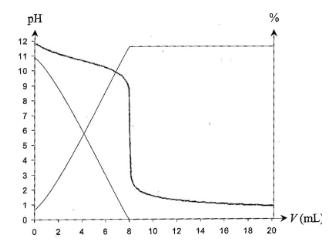
\includegraphics[width=\textwidth]{./Images/mpsi_s18_ex02.png}

\begin{enumerate}
	\item Attribuer les courbes de pourcentage aux espèces correspondantes et déterminer simplement le $pKa$ du couple.
	\item Écrire l'équation de la réaction. Calculer sa constante d'équilibre et justifier qu'elle peut servir de support de titrage.
	\item Justifier qualitativement l'allure de la courbe de $pH$.
	\item Proposer un indicateur coloré adapté au repérage de l'équivalence.
	\item Déterminer la formule de l'amine.
\end{enumerate}

\e{Données :}
\begin{enumerate}
	\item Masses molaires : $M_H = \SI{1.0}{\gram\per\mol}$, $M_C = \SI{12.0}{\gram\per\mol}$, $M_N = \SI{14.0}{\gram\per\mol}$.
	\item Zones de virage d'indicateurs colorés : phénolphtaléine $8.2$ à $10.2$, bleu de bromothymol $6.0$ à $7.6$, vert malachite $0.2$ à $1.8$.
\end{enumerate}

\e{Réponses :}
pKa = 10.7. n = 4.

\subsection{Exercice 3 : Titrage de l'acide acrylique}

On souhaite vérifier la concentration d'une solution d'acide acrylique noté \ce{AH} un peu ancienne (notée $S_0$). Il est écrit sur l'étiquette : $C_0 = \SI{6.25e-1}{\mol\per\liter}$. Pour cela, on décide de réaliser un titrage acido-basique.
On dispose d'une solution titrante de soude (\ce{Na+}, \ce{HO-}) de concentration $C_T = \SI{5.00e-2}{\mol\per\liter}$.

Avant dosage, la solution d'acide acrylique est diluée exactement vingt fois pour obtenir la solution $(S)$. Une prise d'essai $V_2 = \SI{20.0}{mL}$ de la solution $(S)$ est diluée par ajout d'un volume de $\SI{50}{mL}$ d'eau distillée, puis titrée par la solution  d'hydroxyde de sodium.

On note $V_0$ le volume total initial de la solution titrée, $V_T$ le volume de solution titrante ajouté et $V_E$ le volume versé à l’équivalence. Le titrage est suivi par pH-métrie. La courbe $pH = f(V_T)$  est donnée ci dessous.

On donne : $pKa(\ce{AH}/\ce{A-}) = 4.25$.

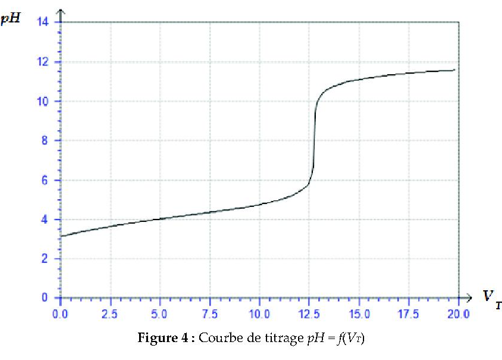
\includegraphics[width=\textwidth]{./Images/mpsi_s18_ex03.png}

\begin{enumerate}
	\item Écrire la réaction de dosage ainsi que la relation à l'équivalence.
	\item Calculer, en considérant que la concentration marquée sur l'étiquette est bonne, le $pH$ de la solution d'acide acrylique dans le bécher avant le début du titrage. Comparer à la valeur lue sur la courbe.
	\item Réciproquement, évaluer la vraie concentration en acide acrylique dans la solution $S$ à partir de la lecture du $pH$ à $V_T = 0$. Pourquoi n'utilise-t-on pas une seule mesure de $pH$, à la place d'un titrage, pour déterminer la concentration en acide acrylique dans la solution $S$ ?
	\item Déterminer la concentration en acide acrylique dans la solution $S$.
\end{enumerate}


\chapter{MPI}

\section{Semaine 02 (23/09-27/09) }


\e{Notions abordées :}
\begin{itemize}
	\item Révisions de MPSI en électronique.
	\item Filtrage d'un signal périodique.
\end{itemize}

\subsection{Exercice 1}

\begin{minipage}[c]{\linewidth/3}
	\begin{circuitikz}
		%Circuit
		\draw (0, 0) 
		to[R, l=$R$] (3, 0)
		to [L, l=$L$, v<=$v_s$] ++ (0, -2)
		-- (0, -2)
		to [open, v=$v_e$] (0, 0);
	\end{circuitikz}
\end{minipage}%
\begin{minipage}[c]{\linewidth/2}
	On donne $R = \SI{1.0}{k\Omega}$ et $L = \SI{10}{mH}$.
	\begin{enumerate}
		\item Quel type de filtre ce circuit permet-il de réaliser ?
		\item Déterminer sa fonction de transfert.
		\item Déterminer les pentes des asymptotes en gain BF et HF.
		\item $v_e$ s'écrit comme somme de trois harmoniques de même amplitude, de même phase à l'origine et de fréquences respectives $f_1 = \SI{100}{Hz}$, $f_2 = \SI{1}{kHz}$ et $f_3 = \SI{100}{kHz}$. Écrire $v_e$ puis $v_s$.
		\item $v_e$ est maintenant un triangle de fréquence \SI{60}{Hz}. Quelle est la forme de $v_s$ ?
	\end{enumerate}
\end{minipage}

\subsection{Exercice 2}

\begin{minipage}[c]{\linewidth/2}
	\begin{circuitikz}
		%Circuit
		\draw (0, 0) 
		to[R, l=$R$] (3, 0)
		to[C, l=$C$] ++(2, 0)
		to [L, l=$L$, v<=$v_s$] ++ (0, -2)
		-- (0, -2)
		to [open, v=$v_e$] (0, 0);
	\end{circuitikz}
\end{minipage}%
\begin{minipage}[c]{\linewidth/2}
	\begin{enumerate}
		\item Quel type de filtre ce circuit permet-il de réaliser ?
		\item Déterminer sa fonction de transfert.
		\item Déterminer les pentes des asymptotes en gain BF et HF. Tracer le diagramme de Bode asymptotique.
		\item $v_e$ s'écrit comme somme de trois harmoniques de même amplitude, de même phase à l'origine et de fréquences respectives $f_1 = \SI{100}{Hz}$, $f_2 = \SI{1}{kHz}$ et $f_3 = \SI{100}{kHz}$. Écrire $v_e$ puis $v_s$.
		\item Ce filtre peut-il avoir un comportement dérivateur ? Intégrateur ?
	\end{enumerate}
\end{minipage}

\subsection{Exercice 3}

\begin{minipage}[c]{\linewidth/2}
	\begin{circuitikz}
		%Circuit
		\draw (0, 0) 
		to[R, l=$R$] (2, 0)
		to[C, l=$C$] ++(2, 0)
		to [R, l=$R$] ++ (0, -2)
		-- (0, -2)
		to [open, v=$v_e$] (0, 0);
		\draw (4, 0)
		-- (6, 0)
		to [C, l=$C$, v<=$v_s$] ++ (0, -2)
		-- (4, -2)
		;
	\end{circuitikz}
\end{minipage}%
\begin{minipage}[c]{\linewidth/2}
	On donne $R = \SI{1.0}{k\Omega}$ et $C = \SI{500}{nF}$.
	\begin{enumerate}
		\item Quel type de filtre ce circuit permet-il de réaliser ?
		\item Déterminer sa fonction de transfert.
		\item Déterminer la bande passante. Définir le facteur de qualité.
		\item $v_e$ s'écrit comme somme de trois harmoniques de même amplitude, de même phase à l'origine et de fréquences respectives $f_1 = \SI{100}{Hz}$, $f_2 = \SI{1}{kHz}$ et $f_3 = \SI{100}{kHz}$. Écrire $v_e$ puis $v_s$.
	\end{enumerate}
\end{minipage}


\section{Semaine 03 (30/09-04/10) }


\e{Notions abordées :}
\begin{itemize}
	\item Électronique de MPSI.
	\item Filtrage d'un signal périodique.
	\item Numérisation.
	\item Portes logiques.
\end{itemize}

\subsection{Exercice 1 : Intégration d'un créneau par un filtre passe bande}

Une tension créneau est injectée dans un filtre passe-bande non inverseur d'ordre 2, de pulsation de résonance $\omega_0$, de facteur de qualité $Q$ et de gain maximum $G_0$. La pulsation $\omega$ de la tension créneau est supposée grande devant $\omega_0$.

\begin{enumerate}
	\item Écrire la fonction de transfert du filtre.
	\item Montrer que ce filtre se comporte vis-à-vis du créneau d'entrée comme un intégrateur.
	\item Écrire l'équation différentielle reliant la tension d'entrée $v_e(t)$ et la tension de sortie $v_s(t)$ de l'intégrateur. Qu'obtient-on précisément en sortie du filtre ? Comment seraient modifiés les résultats si on ajoutait une tension continue au créneau à l'entrée ?
\end{enumerate}

\subsection{Exercice 2 : Shannon comme au cinéma}

Au cinéma, lorsqu'on regarde les roues d'une voiture qui démarre, on les voit d'abord tourner dans le sens réel puis elles semblent tourner à l'envers. Expliquer d'où provient cette illusion. Qu'observe-t-on en visionnant le film lorsque les roues de la voiture tournent à $f_1=\SI{1200}{tours/min}$ ? Et à $f_2 = \SI{1680}{tours/min}$.


\section{Semaine 04 (07/10-11/10) }


\e{Notions abordées :}
\begin{itemize}
	\item Électrocinétique.
	\item Mécanique de MPSI.
\end{itemize}

\subsection{Exercice 1 : Système à deux ressorts}

On considère une masse $m$ astreinte à se déplacer sur un axe horizontal $(Ox)$ et fixée à une paroi à gauche et une à droite par deux ressorts identiques $(k, l_0)$. Les parois sont distantes de $L$.

\begin{enumerate}
	\item Appliquer le principe fondamental de la dynamique à la masse $m$.
	\item En déduire la position d'équilibre $x_e$.
	\item Étudier les petites oscillations autour de la position d'équilibre.
	\item On envisage l'existence d'un frottement fluide d'intensité proportionnelle à la vitesse via une constante $\beta$. Établir l'équation différentielle du mouvement. Pour quelles valeurs de $\beta$ la masse $m$ oscille-t-elle ?
	\item Comment choisir $\beta$ pour un retour le plus rapide à la position d'équilibre. Quel est le temps caractéristique d'amortissement ?
\end{enumerate}

\subsection{Exercice 2 : Frottement et facteur de qualité}

On considère un ressort horizontal de constante de raideur $k$ et de longueur à vide $l_0$. Une extrémité du ressort est fixe et l'autre attachée à un mobile de masse $m$. Le mobile subit une force de frottement fluide proportionnelle à sa vitesse via une constante $\beta$.

\begin{enumerate}
	\item Déterminer l'équation différentielle du mouvement. Introduire une pulsation propre et un facteur de qualité.
	\item Résoudre l'équation différentielle. Simplifier l'expression dans le cas $Q \gg 1$.
	\item En déduire que $Q$ est une bonne approximation du nombre d'oscillations avant le retour à l'équilibre.
	\item On considère maintenant l'énergie mécanique relative perdue sur une pseudo-période. L'exprimer en fonction de $Q$. 
	\item On considère maintenant un opérateur qui impose une force $\vec{F(t)} = m A \cos{\omega t} \vec{e_x}$. Déterminer la fonction de transfert du système et interpréter $Q$ d'une nouvelle façon.
\end{enumerate}

\subsection{Exercice 3 : Mouvement autour d'une position d'équilibre}

Soit un point matériel de masse $m$ astreint à se déplacer selon un axe $(Ox)$ et d'énergie potentielle $E_p(x) = \frac{-a}{x^2} + \frac{b}{x^3}$ avec $a, b > 0$.

\begin{enumerate}
	\item Montrer en général qu'une position d'équilibre correspond à un extremum local d'énergie potentiel. À quelle condition une position d'équilibre est-elle stable ? instable ?
	\item Tracer le profil d'énergie potentiel.
	\item Déterminer la ou les position(s) d'équilibre ainsi que leur stabilité.
	\item Étudier les petites oscillations autour de la position d'équilibre stable.
	\item Déterminer, dans le cas d'une énergie potentielle générale, l'expression de la pulsation des petites oscillations.
\end{enumerate}

\section{Semaine 04 (14/10-18/10) }


\e{Notions abordées :}
\begin{itemize}
	\item Mécanique de MPSI (forces centrales).
	\item Dynamique en référentiel non galiléen.
\end{itemize}

\subsection{Exercice 1 : Force en $1/r^4$}

On considère un point matériel de masse $m$ soumis à la force $\vec{F} = \frac{-K}{r^4} \vec{e}_r$, avec $K>0$.

\begin{enumerate}
	\item Montrer que le mouvement est plan et qu'il vérifie la loi des aires.
	\item Définir une énergie potentielle effective et la tracer.
	\item Discuter graphiquement les trajectoires possibles. Justifier. Existe-t-il une trajectoire circulaire ?
\end{enumerate}

\subsection{Exercice 2 : Satellite géostationnaire}

\begin{enumerate}
	\item Définir un satellite géostationnaire et déterminer son orbite. Justifier.
	\item Quel travail faut il fournir pour l'élever en altitude de $\SI{50}{km}$ ? 
	\item L'essence à une énergie spécifique de $\SI{13.1}{kWh/kg}$ et une masse volumique de $\SI{745}{\kilogram\per\cubic\meter}$. En déduire le volume de carburant nécessaire pour effectuer la manœuvre.
\end{enumerate}

\e{Réponses :}
\begin{enumerate}
	\item $\SI{42e3}{km}$
	\item $\SI{5.7e6}{J}$
	\item $\SI{0.13}{kg}$ et $\SI{0.16}{\liter}$.
\end{enumerate}

\subsection{Exercice 3 : Chute d'un satellite dans l'atmosphère}

\begin{enumerate}
	\item Un satellite est en orbite circulaire autour de la Terre. Montrer qu'il existe une relation simple entre $E_c$ et $E_p$. Exprimer l'énergie mécanique en fonction de $r$.
	\item Comment évolue la vitesse d'un satellite freiné par l'atmosphère ?
	\item Son altitude est $h=\SI{180}{km}$ et la force de frottement a pour norme $\beta m v^2 / h$.
	\begin{enumerate}
		\item Préciser l'unité de $\beta$.
		\item Déterminer la variation d'altitude $\Delta h$ après une révolution. On proposera les hypothèses appropriées.
	\end{enumerate}
\end{enumerate}

\e{Réponse :} $\Delta h = \SI{-28.3}{m}$.

\subsection{Exercice 4 : Pendule pesant dans une voiture accélérée}

Une tige homogène de longueur $l$ et de masse totale $m$ est accrochée en un point $A$ du plafond d'une voiture. La voiture est en translation rectiligne d'accélération $a$ par rapport au référentiel terrestre supposé galiléen. 

Le moment d'inertie de la tige par rapport au point $A$ est $J = \frac{1}{3}m l ^2$. On admet que le point d'application de la force d'inertie d'entraînement est le centre d'inertie de la tige.

\begin{enumerate}
	\item Déterminer l'angle d'équilibre du pendule dans le référentiel de la voiture.
	\item Déterminer la période $T$ des petites oscillations du pendule autour de la position d'équilibre.
\end{enumerate}

\subsection{Exercice 5 : Limite de Roche}

\begin{minipage}[c]{\linewidth/2}
	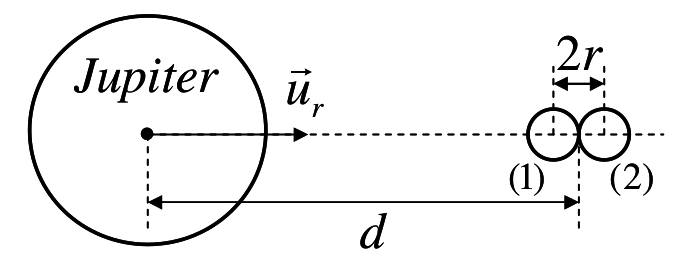
\includegraphics[width=\linewidth]{Images/mp_s04_ex02.png}
\end{minipage}%
\begin{minipage}[c]{\linewidth/2}
	On cherche à déterminer la distance en dessous de laquelle une comète s'approchant de Jupiter se sépare en plusieurs morceaux sous l'effet des forces de marée dues à Jupiter.
	
	On modélise la comète par deux sphères identiques de masses $m$ et de rayon $r$, alignées comme sur le dessin. On suppose que la comète est en orbite circulaire de rayon $d$ autour de Jupiter.
\end{minipage} 

\begin{enumerate}
	\item Montrer que le mouvement du centre d'inertie de la comète est uniforme. Quelle est la nature du mouvement du référentiel barycentrique de la comète par rapport au référentiel de Jupiter ?
	\item Soit $\vec{R}$ la réaction de la sphère $(1)$ sur la sphère $(2)$. Dans le référentiel de la comète, appliquer le PFD à une des deux sphères.
	\item À quelle condition le contact entre les sphères est-il rompu ? Déterminer, sachant que $r \ll d$, la distance limite $d_{lim}$ en dessous de laquelle il ne peut exister de comètes.
\end{enumerate}

\e{Données :} $M_J = \SI{1.9e27}{kg}$, $R_J = \SI{7.1e4}{km}$ et masse volumique de la comète $\rho_c = \SI{1.0e3}{\kilogram\per\cubic\metre}$.

\e{Réponse :} $d_{lim} = \SI{1.8e5}{km}$.

\subsection{Exercice 6 : Usure d'une ligne de TGV}

Un train grande vitesse se dirige vers le sud, depuis Paris (latitude $48.8$°). On considère son mouvement dans le référentiel terrestre non galiléen. Montrer qu'apparaît une réaction horizontale de la voie sur le train. La comparer à la réaction verticale. 


\subsection{Exercice 7 : Impesanteur}

Existe-t-il un endroit où $\vec{g} = \vec{0}$ ? Commenter la valeur numérique obtenue.

\e{Réponse :} $\SI{42e3}{km}$
\section{Semaine 06 (04/11-08/11) }


\e{Notions abordées :}
\begin{itemize}
	\item Mécanique de MPSI.
	\item Dynamique en référentiel non galiléen.
	\item Lois du frottement de Coulomb.
\end{itemize}

\subsection{Exercice 1 : Glissement d'une caisse dans un camion}

\begin{minipage}[c]{\linewidth/2}
	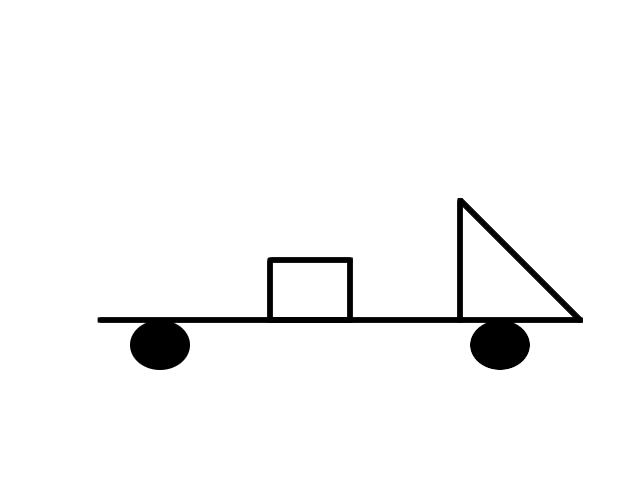
\includegraphics{/home/chams/Documents/Travail/2024-2025/Colles/Images/mp_s05_ex01.png}
\end{minipage}%
\begin{minipage}[c]{\linewidth/2}
	Le camion accélère avec l'accélération constante $a$.
	\begin{enumerate}
		\item À quelle condition le glissement commence-t-il ?
		\item Au bout de combien de temps la caisse atteint-elle le rebord ?
		\item Quelle distance parcourt-elle après être tombée ?
		\item La caisse glisse-t-elle ou bascule-t-elle lors de l'accélération ?
	\end{enumerate}
\end{minipage}

\subsection{Exercice 2 : Cube sur un plan incliné}

Un cube repose sur un plan incliné d'un angle $\alpha$. On augmente $\alpha$ très lentement.

\begin{enumerate}
	\item À quelle condition le glissement commence-t-il ?
	\item À quelle condition le cube bascule-t-il ?
	\item Qu'est ce qui arrive en premier ? On donne le coefficient de frottement bois-bois $f = 0.4$.
\end{enumerate}

\subsection{Exercice 3 : Glissement et liaison avec une corde}

\begin{minipage}[c]{\linewidth/2}
	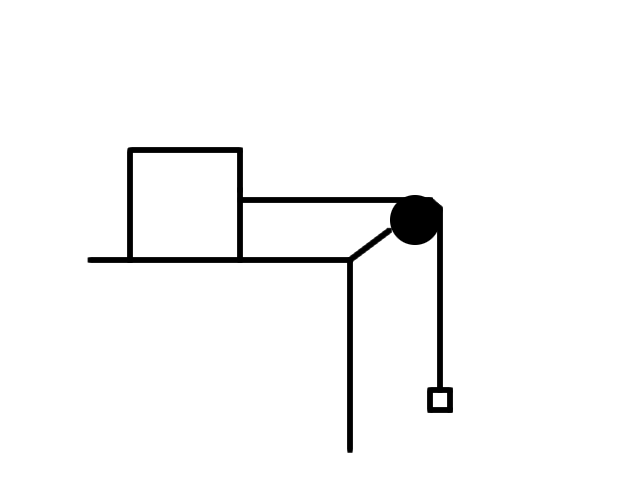
\includegraphics{/home/chams/Documents/Travail/2024-2025/Colles/Images/mp_s05_ex03.png}
\end{minipage}%
\begin{minipage}[c]{\linewidth/2}
	Deux caisses sont liées par une corde qui passe par une poulie. On prend en compte le frottement de la grosse caisse sur la surface. En précisant les hypothèses utilisées, déterminer l'altitude de la caisse suspendue en fonction du temps.
\end{minipage}
\section{Semaine 07 (11/11-15/11) }


\e{Notions abordées :}
\begin{itemize}
	\item Transformations chimiques d'un système.
	\item Acides et bases, réactions acide-base.
\end{itemize}

\subsection{Questions de cours :}
\begin{enumerate}
	\item Une mole de méthane réagit avec une mole de dioxygène selon une réaction de combustion. Déterminer la composition finale du système.
	\item Exprimer l'activité d'une espèce chimique pure, en phase condensée ou très diluée en solution aqueuse.
	\item Exprimer le quotient réactionnel d'une réaction donnée et prévoir le sens d'évolution spontanée d'un système chimique.
\end{enumerate}

\subsection{Exercice 1 : Fluoration du dioxyde d'uranium}

Le dioxyde d'uranium solide réagit avec le fluorure d'hydrogène gazeux pour former du tétrafluorure d'uranium solide et de la vapeur d'eau. 

On maintient la température égale à $\SI{700}{K}$ et la pression totale à $\SI{1}{bar}$. La constante d'équilibre à $\SI{700}{K}$ est égale à $K^\circ = 6.8\times10^4$.

\begin{enumerate}
	\item Écrire la réaction.
	\item On part de $\SI{1.0}{mol}$ de dioxyde d'uranium et de $\SI{1.0}{mol}$ de fluorure d'hydrogène. Quelle sera la composition finale du système ?
	\item Même question en partant de $\SI{0.10}{mol}$ de dioxyde d'uranium et de $\SI{1.0}{mol}$ de fluorure d'hydrogène. Que remarque-t-on dans ce cas ?  
\end{enumerate}

\e{Réponses :}
\begin{enumerate}
	\item -
	\item $\xi = \SI{0.24}{mol}$.
	\item - 
\end{enumerate}

\subsection{Exercice 2 : Constante d'équilibre et quotient de réaction.}

Pour préparer industriellement du dihydrogène, on fait réagir en phase gazeuse du méthane avec de l'eau. La réaction produit également du monoxyde de carbone.

La réaction se déroule sous une pression totale constante $p_{tot} = \SI{10}{bar}$. La constante d'équilibre vaut $K^\circ = 15$. Initialement, le système contient $\SI{10}{mol}$ de méthane, $\SI{30}{mol}$ d'eau, $\SI{5}{mol}$ de monoxyde de carbone et $\SI{15}{mol}$ de dihydrogène. 

\begin{enumerate}
	\item Exprimer la constante d'équilibre en fonction des pressions partielles des constituants.
	\item Exprimer le quotient de réaction $Q$ en fonction de la quantité de matière de chacun des constituants et de la pression totale. Calculer $Q$ dans l'état initial.
	\item Le système est-il à l'équilibre thermodynamique ? Si non, dans quel sens se produira l'évolution ?
	\item Déterminer la composition du système à l'équilibre.
\end{enumerate}

\e{Réponses :}
\begin{enumerate}
	\item -
	\item $Q = 1.56$.
	\item -
	\item $\xi = \SI{3.6}{mol}$.
\end{enumerate}

\subsection{Exercice 3 : Utilisation du quotient de réaction.}

Un récipient de volume $V_0 = \SI{2.00}{L}$ contient initialement $\SI{0.500}{mol}$ de COBr$_2$ qui se décompose à une température de $\SI{346}{K}$ selon la réaction : $$\ce{COBr2_{(g)} = CO_{(g)} + Br2_{(g)}}$$.

\begin{enumerate}
	\item Déterminer la composition du système à l'équilibre sachant que la constante d'équilibre à $\SI{346}{K}$ vaut $K^\circ = 5.46$.
	\item Calculer le pourcentage de COBr$_2$ décomposé à cette température.
	\item L'équilibre précédent étant réalisé, on ajoute $\SI{2.00}{mol}$ de monoxyde de carbone. L'équilibre chimique est-il réalisé ? Si non, décrire l'évolution ultérieure du système.
\end{enumerate}

\e{Réponses :}
\begin{enumerate}
	\item $\xi = \SI{0.285}{mol}$.
	\item 57 \%.
	\item $Q = 43.2$, $\xi' = \SI{0.077}{mol}$.
\end{enumerate}
\section{Semaine 08 (18/11-22/11) }


\e{Notions abordées :}
\begin{itemize}
	\item Transformations chimiques d'un système.
	\item Acides et bases, réactions acide-base.
	\item Réaction d'oxydoréduction et piles.
	\item Dosages.
\end{itemize}

\subsection{Questions de cours}

\begin{enumerate}
	\item Réaliser le schéma d'une pile. 
	\item Écrire une réaction d'oxydoréduction entre l'ion cuivre au degré d'oxydation $2$ et l'argent solide.
	\item Écrire l'équation d'une réaction acide-base et déterminer la valeur de sa constante thermodynamique d'équilibre en fonction des $pKa$ des couples mis en jeu.
\end{enumerate}

\subsection{Exercice 1 : Vitamine C}

La vitamine C, aussi appelée acide ascorbique, est un diacide noté $AscH_2$.

\begin{enumerate}
	\item Dresser le diagramme de prédominance des espèces acido-basiques issues de l'acide ascorbique en fonction du $pH$ de la solution.
	\item On dissout dans l'eau un comprimé contenant $\SI{500}{mg}$ d'acide ascorbique dans une fiole jaugée de volume $V = \SI{200}{mL}$. Déterminer l'état d'équilibre de la solution obtenue.
	\item La vitamine C existe aussi en comprimé tamponné, réalisée en mélangeant l'acide ascorbique $AscH_2$ et de l'ascorbate de sodium $AscHNa$. Un comprimé de vitamine C tamponnée de masse $m$ en principe actif (acide ascorbique sous ses deux formes, diacide et monoacide) est dissous dans $V'=\SI{100}{mL}$ d'eau distillée. La solution obtenue a un $pH$ égal à $4.4$. Déterminer la masse d'acide ascorbique et la masse d'ascorbate de sodium contenues dans ce cachet. On prendra $m=\SI{500}{mg}$ pour les applications numériques.
\end{enumerate}

\e{Données :} 
\begin{itemize}
	\item Les deux $pKa$ associés à l'espèce étudiée sont $4.2$ et $11.6$.
	\item $M(AscH_2) = \SI{176}{\gram \per \mol}$, $M(AscHNa) = \SI{198}{\gram \per \mol}$.
	\item S'il y a plusieurs réactions possibles, on se concentrera sur celle dont la constante thermodynamique est la plus élevée (réaction prépondérante).
\end{itemize} 

\e{Réponses :}
\begin{enumerate}
	\item -
	\item $[AscH_2] = \SI{1.4e-2}{\mol\per\liter}$, $[AscH_-] = [H_3O^+] = \SI{9.4e-4}{\mol\per\liter}$
	\item $m_a = \SI{1.9e2}{mg}$, $m_b=\SI{3.4e2}{mg}$.
\end{enumerate}

\subsection{Exercice 2 : Titrage du dioxyde de soufre dans le vin}

La concentration en masse de dioxyde de soufre dans un vin blanc ne doit pas excéder $\SI{210}{\milli\gram\per\liter}$. Pour vérifier la conformité de la concentration en dioxyde de soufre d'un vin blanc, on utilise une solution titrante de concentration $C_1 = \SI{7.80e-3}{\mol\per\liter}$ en diiode. Dans un erlenmeyer, on verse un volume $V_2 = \SI{25.0}{mL}$ de vin blanc. On ajoute $\SI{2}{mL}$ d'acide sulfurique pour acidifier le milieu. Lors du titrage du vin blanc, l'équivalence est obtenue après avoir versé un volume $V_E = \SI{6.1}{mL}$ de solution titrante. La réaction support du titrage s'écrit $$\ce{SO2(aq) + I2(aq) + 2H2O(l) \rightarrow SO4^{2-}(aq) + 2I-(aq) + 4H+(aq)}$$

Ce vin est il conforme à la législation ?

\e{Donnée :} $M(SO_2) = \SI{64.1}{g\per\mol}$

\e{Réponse :} $\SI{120}{mg/L} < \SI{210}{mg/L}$.

\subsection{Exercice 3 : Pile à combustible}

Dans certaines piles à combustible, on utilise le dihydrogène comme combustible et le dioxygène comme comburant. 

\begin{enumerate}
	\item Écrire la réaction de combustion du dihydrogène par le dioxygène.
	\item Cette réaction est en fait l'association de deux demi-équations d'oxydoréduction mettant en jeu les couples \ce{H^+/H2_{(g)}} et \ce{O2_{(g)}/H2O}. Écrire les demi-équations d'oxydoréduction.
	\item Les deux demi-réactions ont lieu sur deux électrodes. Indiquer la réaction cathodique et la réaction anodique.
	\item Donner l'expression du potentiel d'oxydoréduction pour les deux couples.
	\item Exprimer la constante d'équilibre $K^o$ en fonction des potentiels standards des couples. Calculer sa valeur. Commenter.
\end{enumerate}

\e{Données :} $E^o(H^+, H_2) = 0.00~V$, $E^o(O_2, H_2O) = 1.23~V$.
\section{Semaine 09 (25/11-29/11) }


\e{Notions abordées :}
\begin{itemize}
	\item Transformations chimiques d'un système.
	\item Acides et bases, réactions acide-base.
	\item Réaction d'oxydoréduction et piles.
	\item Dosages.
\end{itemize}

\subsection{Questions de cours}

\begin{enumerate}
	\item Réaliser le schéma d'une pile. 
	\item Écrire une réaction d'oxydoréduction entre l'ion cuivre au degré d'oxydation $2$ et l'argent solide.
	\item Écrire l'équation d'une réaction acide-base et déterminer la valeur de sa constante thermodynamique d'équilibre en fonction des $pKa$ des couples mis en jeu.
\end{enumerate}

\e{Exercices : Cf semaine précédente}
\section{Semaine 10 (02/12-06/12) }


\e{Notions abordées :}
\begin{itemize}
	\item Révisions d'optique géométrique (cf MPSI).
	\item Phénomènes ondulatoires (cf MPSI).
\end{itemize}
\section{Semaine 11 (09/12-13/12) }


\e{Notions abordées :}
\begin{itemize}
	\item Interférences lumineuses.
	\item Sources élargies spatialement et spectralement.
	\item (Pas de Michelson).
\end{itemize}

\subsection{Exercice 1 : Cohérence spatiale des fentes d'Young}

Quelle est la largeur d'une source étendue qui provoque un brouillage de la figure d'interférence dans le cas des fentes d'Young ?

\subsection{Exercice 2 : Interférences sur une goutte}

On considère une goutte liquide d'indice $n=\SI{1.4}{}$ sur un solide réfléchissant, éclairée en incidence normale par une source monochromatique de longueur d'onde $\lambda = \SI{546}{nm}$. La goutte est assimilable à une portion de sphère de centre $C$. Son diamètre dans le plan de contact est $d=\SI{0.5}{mm}$ et l'angle de contact à son bord est $\theta = \SI{5}{\degree}$. 

\begin{enumerate}
	\item Justifier que l'on peut négliger la réfraction à la surface de la goutte.
	\item Justifier que des interférences lumineuses apparaissent. Où sont elles localisées ?
	\item Calculer la différence de marche à la surface de la goutte, à une distance $r$ de l'axe de révolution.
	\item Déterminer les rayons des anneaux brillants successifs.
	\item Déterminer l'ordre d'interférence au centre, et au bord. En déduire le nombre d'anneaux visibles.
\end{enumerate}

\e{Réponse :} Au premier ordre en $\theta$, $N = 1 + \lfloor \frac{n d \theta}{2 \lambda}\rfloor = \SI{52}{anneaux}$. (à vérifier)

\subsection{Exercice 3 : Mesure de l'indice d'un verre}

On considère le dispositif des fentes d'Young avec lentille éclairé par une source ponctuelle monochromatique au foyer objet d'une lentille convergente. Devant l'une des deux fentes, on place une lame de verre d'épaisseur $e$ connue et d'indice $n$ inconnu.

\begin{enumerate}
	\item Décrire la figure d'interférences. Peut-on déterminer l'indice du verre ?
	\item Montrer qualitativement que l'on peut déterminer l'indice du verre en passant en lumière blanche.
	\item Le montrer quantitativement en considérant une source lumineuse de distribution spectrale d'intensité $\frac{dI}{d\nu}$ homogène, de fréquence centrale $\nu_0$ et de largeur $\Delta \nu$.
\end{enumerate}
\section{Semaine 12 (16/12-20/12) }


\e{Notions abordées :}
\begin{itemize}
	\item Interférences lumineuses (cf semaine précédente).
	\item Interféromètre de Michelson en lame d'air.
\end{itemize}

\subsection{Exercice 1 : Interférences sur une goutte}

On considère une goutte liquide d'indice $n=\SI{1.4}{}$ sur un solide réfléchissant, éclairée en incidence normale par une source monochromatique de longueur d'onde $\lambda = \SI{546}{nm}$. La goutte est assimilable à une portion de sphère de centre $C$. Son diamètre dans le plan de contact est $d=\SI{0.5}{mm}$ et l'angle de contact à son bord est $\theta = \SI{5}{\degree}$. 

\begin{enumerate}
	\item Justifier que l'on peut négliger la réfraction à la surface de la goutte.
	\item Justifier que des interférences lumineuses apparaissent. Où sont elles localisées ?
	\item Calculer la différence de marche à la surface de la goutte, à une distance $r$ de l'axe de révolution.
	\item Déterminer les rayons des anneaux brillants successifs.
	\item Déterminer l'ordre d'interférence au centre, et au bord. En déduire le nombre d'anneaux visibles.
\end{enumerate}

\e{Réponse :} Au premier ordre en $\theta$, $N = 1 + \lfloor \frac{n d \theta}{2 \lambda}\rfloor = \SI{52}{anneaux}$. (à vérifier)

\subsection{Exercice 2 : Mesure de l'épaisseur d'une lame}

On considère un Michelon en lame d'air éclairé en incidence normale et en lumière blanche. En sortie de l'interféromètre, on place un spectromètre connecté à un ordinateur au foyer image d'une lentille convergente.

Dans les bras de l'interféromètre, on place une lame de verre d'indice $n=1.50$ et d'épaisseur $e$.

Sur l'ordinateur, on observe le spectre de la lumière reçue. On remarque que les longueurs d'onde $500.0$, $502.5$, $505.1$, $507.6$, $510.2$ et $512.8$ nm correspondent à des maxima d'intensité.

Expliquer le phénomène observé et en déduire l'épaisseur de la lame.

\e{Réponse :} $e = \SI{0.1}{mm}$.

\subsection{Exercice 3 : Mesure de l'indice de l'air}

Un Michelson est réglé en lame d'air d'épaisseur $e$ et éclairé par une source de lumière quasi-monochromatique de longueur d'onde dans le vide $\lambda_0 = \SI{632}{nm}$. Deux cuves identiques, à faces parallèles et transparentes, de longueur $L=\SI{3.00}{cm}$ sont placées entre la séparatrice et chacun des miroirs. L'écran est placé au foyer image d'une lentille convergente.

Dans la situation initiale, les deux cuves sont pleines d'air à pression atmosphérique. On fait progressivement le vide dans l'une des deux cuves et on voit défiler $26$ franges au centre de l'écran. En déduire l'indice de l'air.

\e{Réponse :} $n_{air} - n_{vide} = \SI{2.7e-4}{}$
\section{Semaine 13 (06/01-10/01)}


\e{Notions abordées :}
\begin{itemize}
	\item Interférences lumineuses.
	\item Interféromètre de Michelson.
\end{itemize}

\subsection{Questions de cours :}
\begin{enumerate}
	\item Déterminer l'expression de la différence de marche pour l'interféromètre de Michelson en lame d'air et décrire la figure d'interférences.
	\item Pour l'interféromètre de Michelson en coin d'air, préciser la localisation des interférences. Expliquer comment les observer. Déterminer l'expression de la différence de marche.
	\item Peut on utiliser une source étendue avec le dispositif des trous d'Young ? Et pour le Michelson en configuration lame d'air ? coin d'air ? Conclusion sur l'intérêt de l'interféromètre de Michelson ?
\end{enumerate}

\subsection{Exercices}
cf semaine précédente
\section{Semaine 14 (13/01-17/01)}


\e{Notions abordées :}
\begin{itemize}
	\item Électrostatique (Gauss et Maxwell-Gauss).
	\item Interféromètre de Michelson.
\end{itemize}

\subsection{Questions de cours :}
\begin{enumerate}
	\item Calculer le champ électrique créé par une plaque infinie de densité de charge $\sigma$ uniforme.
	\item Calculer le champ électrique créé par un cylindre infini de densité de charge $\sigma$ uniforme.
	\item Calculer le champ électrique créé par une boule de densité de charge $\rho$ uniforme.
\end{enumerate}

\subsection{Questions sur le Michelson :}
\begin{enumerate}
	\item Déterminer l'expression de la différence de marche pour l'interféromètre de Michelson en lame d'air et décrire la figure d'interférences.
	\item Pour l'interféromètre de Michelson en coin d'air, préciser la localisation des interférences. Expliquer comment les observer. Déterminer l'expression de la différence de marche.
	\item Peut on utiliser une source étendue avec le dispositif des trous d'Young ? Et pour le Michelson en configuration lame d'air ? coin d'air ? Conclusion sur l'intérêt de l'interféromètre de Michelson ?
\end{enumerate}

\subsection{Exercices}
cf semaine précédente
\section{Semaine 15 (20/01-24/01)}


\e{Notions abordées :}
\begin{itemize}
	\item Électrostatique.
\end{itemize}

\subsection{Questions de cours}
\begin{enumerate}
	\item Démontrer, à partir du théorème de Gauss, l'équation de Maxwell-Gauss.
	\item Exprimer, à partir du théorème de Gauss, le champ électrique généré par une charge ponctuelle $q$.
	\item Exprimer la capacité d'un condensateur plan.
\end{enumerate}

\subsection{Exercice 1 : Condensateur cylindrique}

On considère deux électrodes cylindriques infinies, de même axe, de rayons $R_1$ et $R_2 = R_1 + e$. Le cylindre central porte la charge surfacique $+\sigma$.

\begin{enumerate}
	\item Quelle est la charge surfacique portée par le cylindre extérieur ?
	\item Sur un schéma, faire figurer les électrodes, leurs dimensions et le champ électrique.
	\item Déterminer l'expression de la capacité d'un tronçon de longueur $H$ du condensateur en fonction des paramètres géométriques et de $\epsilon_0$.
	\item Commenter le cas $e \ll R_1$.
\end{enumerate}

\subsection{Exercice 2 : Plaque épaisse chargée}

On considère une plaque épaisse de largeur et longueur $L$ occupant l'espace entre $z=-a/2$ et $z=+a/2$. Elle porte une charge $Q$ répartie uniformément.

On réalise l'étude au voisinage de $x = 0$ et $y = 0$, ce qui permet de négliger les effets de bords. 

\begin{enumerate}
	\item Déterminer le champ électrique qu'elle génère.
	\item Dans la limite $a \longrightarrow 0$ :
	\begin{enumerate}
		\item Déterminer la charge surfacique $\sigma$.
		\item Déterminer la relation de passage entre $\overrightarrow{E(z=0^+)}$ et $\overrightarrow{E(z=0^-)}$.
	\end{enumerate}
\end{enumerate}

\subsection{Exercice 3 : Condensateur à cylindres parallèles}

On considère deux cylindres infinis identiques, de rayon $a$. Les axes des deux cylindres sont parallèles et distants de $2 D$. Le cylindre $1$ porte la charge surfacique $+\sigma$.

\begin{enumerate}
	\item Quelle est la charge surfacique portée par le deuxième cylindre ?
	\item Sur un schéma, faire figurer les cylindres, leurs dimensions, les charges et le champ électrique.
	\item À l'aide du théorème de superposition, déterminer l'expression de la capacité d'un tronçon de longueur $H$ du condensateur en fonction des paramètres géométriques et de $\epsilon_0$.
\end{enumerate}

\section{Semaine 16 (27/01-31/01)}


\e{Notions abordées :}
\begin{itemize}
	\item Électrostatique (cf. semaine précédente).
	\item Dipôle électrostatique.
	\item Magnétostatique.
\end{itemize}

\subsection{Questions de cours}
\begin{enumerate}
	\item Montrer que le champ magnétique est à flux conservatif. 
	\item Démontrer l'équation de Maxwell-Ampère à partir du théorème d'Ampère.
	\item Déterminer le champ magnétique généré par un fil rectiligne infini et infiniment fin.
\end{enumerate}


\subsection{Exercice 1 : Bobine torique}

On considère une bobine torique de rayon moyen $R$, comportant $N$ spires, de section carrée de côté $a$ et parcourue par un courant $I$. Déterminer le champ magnétique produit en tout point de l'espace. Comparer avec le champ magnétique du solénoïde infini.

\subsection{Exercice 2 : Caractéristiques d'un câble coaxial}

Un câble coaxial est constitué de deux cylindres conducteurs de rayons $R_1$ et $R_2 > R_1$ sur lesquels circulent, en surface, des courants d'intensité $I$ et de sens opposés.

\begin{enumerate}
	\item Déterminer le champ magnétique.
	\item La densité volumique d'énergie magnétique est donnée par $U_m = \frac{\vec{B}^2}{2 \mu_0}$. En déduire l'inductance linéique du câble coaxial.
	\item Les deux cylindres portent également des charges opposées. Reprendre les calculs pour le champ électrique. En déduire la capacité par unité de longueur.
	\item Quelle relation simple trouve-t-on entre l'inductance et la capacité ?
\end{enumerate}

\subsection{Exercice 3 : Équilibre d'une tige dans un champ non uniforme}

Une tige $[OA]$ de masse $m$ et de longueur $L$ est en rotation autour de l'axe $(Ox)$ horizontal. Son moment d'inertie est $J = \frac{1}{3} m L^2$. Elle est parcourue par un courant d'intensité $i$ dirigée de $O$ vers $A$. Son inclinaison par rapport à la verticale est mesurée par l'angle $\theta$. Un fil rectiligne d'axe vertical $(Oz)$ est parcouru par un courant de même intensité $i$ dirigée vers le haut. À l'équilibre de la tige, donner l'expression de $i$ en fonction de $\theta$, $L$, $m$ et $g$. 


\subsection{Exercice 4 : Action mécanique d'un fil sur un autre fil parallèle}

Deux fils rectilignes infinis parallèles sont distants de $d = \SI{1.0}{m}$. Ils sont parcourus par des courants de même intensité $I$ et de même sens. La force subie par un tronçon de longueur $L = \SI{1.0}{m}$ d’un des fils est égale $\SI{2.0e-7}{N}$.

Déterminer la valeur de $I$.
\section{Semaine 17 (03/02-07/02)}


\e{Notions abordées :}
\begin{itemize}
	\item Magnétostatique.
	\item Dipôle magnétique.
	\item Équations de Maxwell.
	\item Révisions d'induction.
\end{itemize}

\subsection{Questions de cours}
\begin{enumerate}
	\item Montrer que le champ magnétique est à flux conservatif. 
	\item Démontrer l'équation de Maxwell-Ampère à partir du théorème d'Ampère.
	\item Donner les équations de Maxwell.
\end{enumerate}


\subsection{Exercice 1 : Un exo d'induction}

\subsection{Exercice 2 : Inductances propres et mutuelles}

\begin{enumerate}
	\item Rappeler la définitions des inductances propres et mutuelles. À quoi ces grandeurs nous servent-elles ?
	\item Calculer l'inductance propre d'un solénoïde de longueur $l$, de section $S$, comportant $N$ spires, et supposé suffisamment long pour négliger les effets de bords. Application numérique pour une bobine de TP.
	\item Exprimer l'énergie magnétique stockée dans la bobine. Retrouver l'expression de la densité volumique d'énergie magnétique.
	\item On considère un petit solénoïde à l'intérieur d'un gros solénoïde, les deux partageant le même axe. Déterminer l'inductance mutuelle.
\end{enumerate}

\e{Réponses :}
\begin{enumerate}
	\item -
	\item $L = \mu_0 \frac{N^2 S}{l}$
	\item -
	\item $M = \mu_0 \frac{N_1 N_2}{l_1}S_1$
\end{enumerate}

\subsection{Exercice 3 : Induction par un aimant mobile}

Une spire circulaire d'axe $(Oz)$, de rayon $a$ et de résistance $R$ est immobile. Sur son axe, on rapproche à vitesse $\vec{V} = V \vec{e_z}$ constante un petit aimant assimilé à un dipôle magnétique de moment $\vec{\mathcal{M}} = \mathcal{M}\vec{e_z}$.

\begin{enumerate}
	\item Prévoir le sens du courant $i$ induit dans la spire.
	\item Calculer le courant $i$ dans la spire.
	\item Quelle est la force exercée par l'aimant sur la spire ? Commenter.
\end{enumerate}
\section{Semaine 18 (10/02-14/02)}


\e{Notions abordées :}
\begin{itemize}
	\item Équations de Maxwell.
	\item Ondes électromagnétiques dans le vide.
	\item Réflexion sur un conducteur parfait.
\end{itemize}

\subsection{Questions de cours}
\begin{enumerate}
	\item Déterminer l'équation de propagation des ondes électromagnétiques dans le vide.
	\item Déterminer l'équation de dispersion des OPPH électromagnétiques dans le vide. Définir vitesse de phase et vitesse de groupe, les calculer.
	\item Démontrer la relation de structure pour une OPPH électromagnétique. Cas du vide.
\end{enumerate}

\subsection{Exercice 1 : Propagation guidée entre deux plans}

Deux plans infinis conducteurs parfaits délimitent une cavité vide entre $z=0$ et $z=b$. 

\begin{enumerate}
	\item Rappeler l'équation de propagation du champ électromagnétique dans la cavité.
	\item Justifier que, contrairement à ce qu'on fait d'habitude, on ne peut pas chercher une solution polarisée suivant $\vec{u_y}$ sous la forme d'une OPPH.
	
	On cherche une solution de l'équation sous la forme $$\vec{E}(x, z, t) = \beta(z)\vec{u_y}\cos(\omega t - k x)$$.
	
	\item Déterminer l'équation différentielle vérifiée par $\beta$. En donner la solution générale.
	\item Montrer que l'onde ne peut exister que si $\omega > kc$. Commenter en relation avec la relation de dispersion habituelle.
	\item Déterminer complètement $\beta(z)$.
	\item Déterminer la relation de dispersion. 
	\item En déduire qu'il existe une pulsation minimale pour qu'une onde électromagnétique se propage dans le guide.
\end{enumerate}

\e{Réponse :} $\vec{k}^2 = \frac{\omega^2}{c^2} - \frac{n^2 \pi^2}{b^2}$

\subsection{Exercice 2 : Lois de Descartes sur la réflexion et la réfraction}

L'objectif de cet exercice est de redémontrer les lois de Descartes à l'interface entre deux diélectriques.

On rappelle que dans un diélectrique, tout se passe comme dans le vide, à condition de remplacer $\epsilon_0$ par $\epsilon = \epsilon_0 \epsilon_r$.

On considère donc deux diélectriques accolés. Le milieu $1$ de permittivité $epsilon_1$ occupe le demi-espace $z<0$. Le milieu $2$ de permittivité $epsilon_2$ occupe le demi-espace $z>0$.

On considère également une OPPH électromagnétique incidente $(\vec{E_i}, \vec{B_i}, \omega_i, \vec{k_i} = k_{i,x}\vec{e_x} + k_{i, z}\vec{e_z})$ provenant du milieu $1$ vers l'interface avec un angle $\alpha$ par rapport à la normale. Pour simplifier, on suppose le champ électrique incident polarisé rectilignement selon la perpendiculaire au plan d'incidence.

On rappelle qu'à une interface, la composante tangentielle du champ électrique est continue.

\begin{enumerate}
	\item Rappeler les trois lois de Descartes.
	
	\item Justifier qu'il doit exister une onde transmise et/ou une onde réflechie. 
	
	On appellera $(\vec{E_t}, \vec{B_t}, \omega_t, \vec{k_t})$ l'onde transmise et $(\vec{E_r}, \vec{B_r}, \omega_r, \vec{k_r})$ l'onde réfléchie. 
	
	\item Justifier qualitativement que, si ils existent, les champ électrique transmis et réfléchi ont la même polarisation que le champ électrique incident.
	
	\item Sur un schéma, faire figurer l'interface, les trois ondes ainsi que les angles respectifs.
	
	\item Montrer que les ondes ont toute la même pulsation.
	
	\item Montrer que les ondes ont toute le même $k_x$.
	
	\item Montrer que $\frac{\vec{k_t}^2}{\epsilon_{r2}} = \frac{\vec{k_r}^2}{\epsilon_{r1}} = \frac{\vec{k_i}^2}{\epsilon_{r1}}$.
	
	\item En déduire les lois de Descartes sur la réflexion et la réfraction.
\end{enumerate}

\subsection{Exercice 3 : Équation de Klein-Gordon et masse du photon}

\begin{enumerate}
	\item Rappeler l'équation de propagation des ondes électromagnétiques dans le vide.
	
	Dans le cadre de la théorie électromagnétique étendue au cas d'un photon de masse non nulle, l'équation de propagation du champ électrique devient $$\Delta \vec{E} - \frac{1}{c^2} \frac{\partial^2 \vec{E}}{\partial t^2} = \eta^2 \vec{E}$$
	
	\item Quelle est l'unité de $\eta$ ?
	\item Déterminer la relation de dispersion.
	\item Exprimer les vitesses de phase et de groupe en fonction de $c$, $\omega$ et $\eta$. Les tracer. Commentaires ?
	\item Rappeler les expressions de l'énergie $E$ et de la quantité de mouvement $\vec{p}$ d'un photon.
	\item Sachant que pour une particule relativiste de masse $m$, on a $E^2 = p^2 c^2 + m^2 c^4$, exprimer la masse du photon en fonction de $\eta$, $\hbar$ et $c$.
	
	Deux photons de longueurs d'ondes $\lambda_1$ et $\lambda_2$ sont émis au même instant par une source ponctuelle située à une distance $L$. On supposera $\eta^2 \lambda_{1, 2}^2 \ll 1$.
	
	\item Exprimer la différence $\delta t$ des temps de réception des deux signaux.
	
	\item L'observation de certaines étoiles doubles donne $\delta t < \SI{1e-3}{s}$ pour $\lambda_1 = \SI{0.4}{\micro\meter}$, $\lambda_2 = \SI{0.8}{\micro\meter}$ et $L = \SI{1e3}{\textrm{années lumières}}$. En déduire une limite supérieure pour la masse du photon. Commentaire.
	
\end{enumerate}



\chapter{MP}
\section{Semaine 01 (16/09-20/09) }


\e{Notions abordées :}
\begin{itemize}
	\item Révisions de MPSI en électronique.
	\item Filtrage d'un signal périodique.
	\item Traitement numérique du signal.
\end{itemize}

\subsection{Exercice 1}

\begin{minipage}[c]{\linewidth/3}
	\begin{circuitikz}
		%Circuit
		\draw (0, 0) 
			to[R, l=$R$] (3, 0)
			to [L, l=$L$, v<=$v_s$] ++ (0, -2)
			-- (0, -2)
			to [open, v=$v_e$] (0, 0);
	\end{circuitikz}
\end{minipage}%
\begin{minipage}[c]{\linewidth/2}
	On donne $R = \SI{1.0}{k\Omega}$ et $L = \SI{10}{mH}$.
	\begin{enumerate}
		\item Quel type de filtre ce circuit permet-il de réaliser ?
		\item Déterminer sa fonction de transfert.
		\item Déterminer les pentes des asymptotes en gain BF et HF.
		\item $v_e$ s'écrit comme somme de trois harmoniques de même amplitude, de même phase à l'origine et de fréquences respectives $f_1 = \SI{100}{Hz}$, $f_2 = \SI{1}{kHz}$ et $f_3 = \SI{100}{kHz}$. Écrire $v_e$ puis $v_s$.
		\item $v_e$ est maintenant un triangle de fréquence \SI{60}{Hz}. Quelle est la forme de $v_s$ ?
	\end{enumerate}
\end{minipage}

\subsection{Exercice 2}

\begin{minipage}[c]{\linewidth/2}
	\begin{circuitikz}
		%Circuit
		\draw (0, 0) 
		to[R, l=$R$] (3, 0)
		to[C, l=$C$] ++(2, 0)
		to [L, l=$L$, v<=$v_s$] ++ (0, -2)
		-- (0, -2)
		to [open, v=$v_e$] (0, 0);
	\end{circuitikz}
\end{minipage}%
\begin{minipage}[c]{\linewidth/2}
	\begin{enumerate}
		\item Quel type de filtre ce circuit permet-il de réaliser ?
		\item Déterminer sa fonction de transfert.
		\item Déterminer les pentes des asymptotes en gain BF et HF. Tracer le diagramme de Bode asymptotique.
		\item $v_e$ s'écrit comme somme de trois harmoniques de même amplitude, de même phase à l'origine et de fréquences respectives $f_1 = \SI{100}{Hz}$, $f_2 = \SI{1}{kHz}$ et $f_3 = \SI{100}{kHz}$. Écrire $v_e$ puis $v_s$.
		\item Ce filtre peut-il avoir un comportement dérivateur ? Intégrateur ?
	\end{enumerate}
\end{minipage}

\subsection{Exercice 3}

\begin{minipage}[c]{\linewidth/2}
	\begin{circuitikz}
		%Circuit
		\draw (0, 0) 
			to[R, l=$R$] (2, 0)
			to[C, l=$C$] ++(2, 0)
			to [R, l=$R$] ++ (0, -2)
			-- (0, -2)
			to [open, v=$v_e$] (0, 0);
		\draw (4, 0)
			-- (6, 0)
			to [C, l=$C$, v<=$v_s$] ++ (0, -2)
			-- (4, -2)
			;
	\end{circuitikz}
\end{minipage}%
\begin{minipage}[c]{\linewidth/2}
	On donne $R = \SI{1.0}{k\Omega}$ et $C = \SI{500}{nF}$.
	\begin{enumerate}
		\item Quel type de filtre ce circuit permet-il de réaliser ?
		\item Déterminer sa fonction de transfert.
		\item Déterminer la bande passante. Définir le facteur de qualité.
		\item $v_e$ s'écrit comme somme de trois harmoniques de même amplitude, de même phase à l'origine et de fréquences respectives $f_1 = \SI{100}{Hz}$, $f_2 = \SI{1}{kHz}$ et $f_3 = \SI{100}{kHz}$. Écrire $v_e$ puis $v_s$.
	\end{enumerate}
\end{minipage}
\section{Semaine 02 (23/09-27/09) }


\e{Notions abordées :}
\begin{itemize}
	\item Mécanique du point.
	\item Traitement numérique du signal.
\end{itemize}

\subsection{Exercice 1}

\begin{enumerate}
	\item Définir un satellite géostationnaire et calculer son altitude.
	\item Quel travail faut il fournir pour augmenter son altitude de $\SI{50}{km}$.
\end{enumerate}

\subsection{Exercice 2}

On considère un point matériel astreint à se déplacer autour d'un anneau en rotation autour d'un diamètre, à $\omega$ constante.

Positions d'équilibre ? Stabilité ?

\subsection{Exercice 3}

On cherche à graver sur un $CD$ une musique. Toutefois, il existe un signal parasite à $f_p = \SI{42.1}{kHz}$. 

\begin{enumerate}
	\item Échantillonnage sur 16 bits. Quelle est la taille du fichier si la durée vaut $74$ minutes.
	\item Le critère de Shannon est il vérifié ? Conséquence ?
	\item Comment résoudre ce problème ?
\end{enumerate}


\subsection{Exercice 4}

Décrire le mouvement d'une particule chargée dans un champ magnétique statique uniforme.

\section{Semaine 03 (30/09-04/10) }

\e{Notions abordées :}
\begin{itemize}
	\item Traitement numérique du signal.
	\item Mécanique de MPSI.
	\item Dynamique en référentiel non galiléen.
\end{itemize}

\subsection{Exercice 1}

Une tige rigide est en rotation uniforme autour de son axe à la pulsation $\omega$. Un mobile M est lié par un fil au point O situé sur l'axe à l'altitude $h$. 

\begin{enumerate}
	\item Démontrer la loi de composition des accélérations pour un référentiel en rotation uniforme.
	\item Déterminer l'angle $\alpha_0$ d'équilibre du mobile.
	\item Étudier la stabilité de la position d'équilibre.
\end{enumerate}

\subsection{Exercice 2}

Un électron et un proton de même énergie cinétique sont plongés dans un champ magnétique uniforme, orthogonal à leur vitesse initiale.

\begin{enumerate}
	\item Décrire qualitativement les trajectoires.
	\item Comparer :
	\begin{itemize}
		\item Leur vitesse.
		\item Le rayon de leur trajectoire.
		\item Leur période.
	\end{itemize}
	\item Calculer la force centrifuge subie par l'électron.
\end{enumerate}

\subsection{Exercice 3}

Un mobile $M$ coulisse sans frottement  sur un axe horizontal $(Ox)$ dans un train qui accélère avec une accélération $A\vec{u_x}$, le point $O$ étant fixé à l'arrière du wagon. Entre $O$ et $M$ on place un ressort $(k, l_0)$. À $t=0$, $x=l_0$ et la vitesse de $M$ dans le référentiel du train est nulle.

\begin{enumerate}
	\item Démontrer la loi de composition des accélérations dans un référentiel uniformément accéléré.
	\item Établir $x(t)$.
\end{enumerate}




\section{Semaine 04 (07/10-11/10) }

\e{Notions abordées :}
\begin{itemize}
	\item Mécanique de MPSI (forces centrales et dynamique du solide).
	\item Dynamique en référentiel non galiléen.
\end{itemize}

\subsection{Exercice 1 : Pendule pesant dans une voiture accélérée}

Une tige homogène de longueur $l$ et de masse totale $m$ est accrochée en un point $A$ du plafond d'une voiture. La voiture est en translation rectiligne d'accélération $a$ par rapport au référentiel terrestre supposé galiléen. 

Le moment d'inertie de la tige par rapport au point $A$ est $J = \frac{1}{3}m l ^2$. On admet que le point d'application de la force d'inertie d'entraînement est le centre d'inertie de la tige.

\begin{enumerate}
	\item Déterminer l'angle d'équilibre du pendule dans le référentiel de la voiture.
	\item Déterminer la période $T$ des petites oscillations du pendule autour de la position d'équilibre.
\end{enumerate}

\subsection{Exercice 2 : Limite de Roche}

\begin{minipage}[c]{\linewidth/2}
	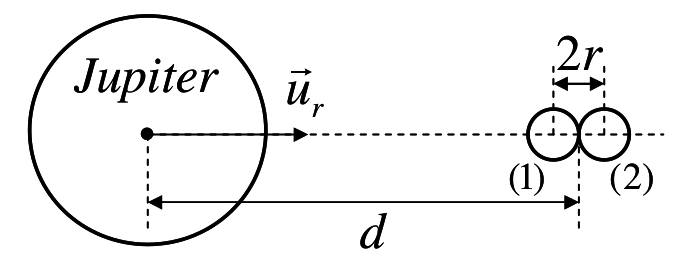
\includegraphics[width=\linewidth]{Images/mp_s04_ex02.png}
\end{minipage}%
\begin{minipage}[c]{\linewidth/2}
	On cherche à déterminer la distance en dessous de laquelle une comète s'approchant de Jupiter se sépare en plusieurs morceaux sous l'effet des forces de marée dues à Jupiter.
	
	On modélise la comète par deux sphères identiques de masses $m$ et de rayon $r$, alignées comme sur le dessin. On suppose que la comète est en orbite circulaire de rayon $d$ autour de Jupiter.
\end{minipage} 

\begin{enumerate}
	\item Montrer que le mouvement du centre d'inertie de la comète est uniforme. Quelle est la nature du mouvement du référentiel de la comète par rapport au référentiel de Jupiter ?
	\item Soit $\vec{R}$ la réaction de la sphère $(1)$ sur la sphère $(2)$. Dans le référentiel de la comète, appliquer le PFD à une des deux sphères.
	\item À quelle condition le contact entre les sphères est-il rompu ? Déterminer, sachant que $r \ll d$, la distance limite $d_{lim}$ en dessous de laquelle il ne peut exister de comètes.
\end{enumerate}

\e{Données :} $M_J = \SI{1.9e27}{kg}$, $R_J = \SI{7.1e4}{km}$ et masse volumique de la comète $\rho_c = \SI{1.0e3}{\kilogram\per\cubic\metre}$.

\e{Réponse :} $d_{lim} = \SI{1.8e5}{km}$.

\subsection{Exercice 3 : Usure d'une ligne de TGV}

Un train grande vitesse se dirige vers le sud, depuis Paris (latitude $48.8$°). On considère son mouvement dans le référentiel terrestre non galiléen. Montrer qu'apparaît une réaction horizontale de la voie sur le train. La comparer à la réaction verticale. 




\section{Semaine 05 (14/10-18/10) }

\e{Notions abordées :}
\begin{itemize}
	\item Mécanique de MPSI (forces centrales et dynamique du solide).
	\item Dynamique en référentiel non galiléen.
	\item Lois du frottement solide.
\end{itemize}

\subsection{Exercice 1 : Glissement d'une caisse dans un camion}

\begin{minipage}[c]{\linewidth/2}
	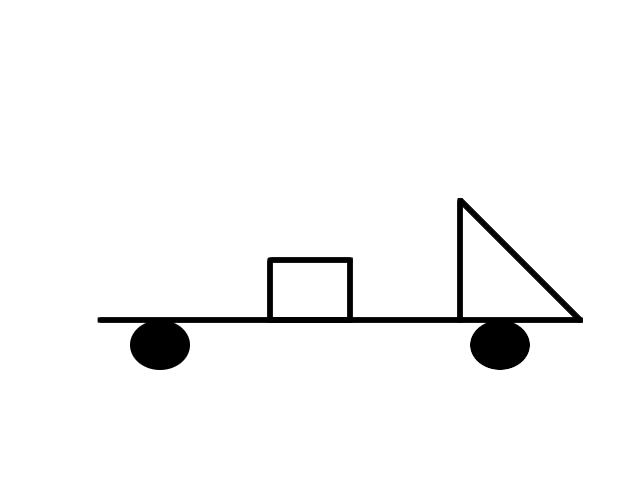
\includegraphics{/home/chams/Documents/Travail/2024-2025/Colles/Images/mp_s05_ex01.png}
\end{minipage}%
\begin{minipage}[c]{\linewidth/2}
	Le camion accélère avec l'accélération constante $a$.
	\begin{enumerate}
		\item À quelle condition le glissement commence-t-il ?
		\item Au bout de combien de temps la caisse atteint-elle le rebord ?
		\item Quelle distance parcourt-elle après être tombée ?
		\item La caisse glisse-t-elle ou bascule-t-elle lors de l'accélération ?
	\end{enumerate}
\end{minipage}

\subsection{Exercice 2 : Cube sur un plan incliné}

Un cube repose sur un plan incliné d'un angle $\alpha$. On augmente $\alpha$ très lentement.

\begin{enumerate}
	\item À quelle condition le glissement commence-t-il ?
	\item À quelle condition le cube bascule-t-il ?
	\item Qu'est ce qui arrive en premier ? On donne le coefficient de frottement bois-bois $f = 0.4$.
\end{enumerate}

\subsection{Exercice 3 : Glissement et liaison avec une corde}

\begin{minipage}[c]{\linewidth/2}
	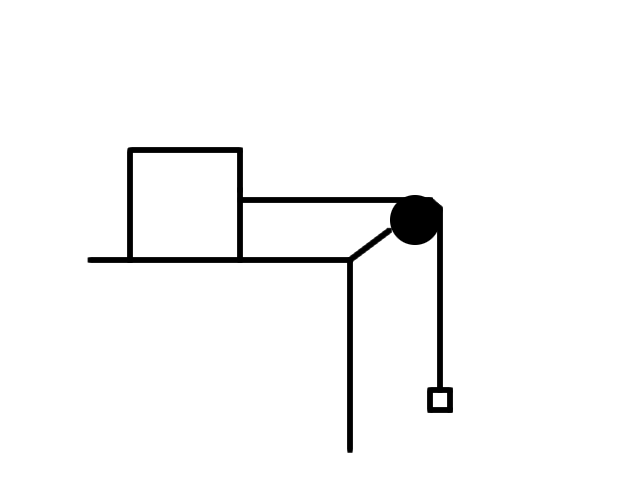
\includegraphics{/home/chams/Documents/Travail/2024-2025/Colles/Images/mp_s05_ex03.png}
\end{minipage}%
\begin{minipage}[c]{\linewidth/2}
	Deux caisses sont liées par une corde qui passe par une poulie. On prend en compte le frottement de la grosse caisse sur la surface. En précisant les hypothèses utilisées, déterminer l'altitude de la caisse suspendue en fonction du temps.
\end{minipage}



\section{Semaine 06 (04/11-08/11) }

\e{Notions abordées :}
\begin{itemize}
	\item Particules dans un $\vec{E}, \vec{B}$ statique (MPSI).
	\item Électrostatique :
	\begin{itemize}
		\item Distributions de charges et de courants.
		\item Symétries et invariances.
		\item Loi de Coulomb.
		\item Théorème de Gauss.
		\item Analogie gravitationnelle.
	\end{itemize}
\end{itemize}

\subsection{Exercice 1 : Condensateur cylindrique}

Deux cylindres métalliques $\mathcal{C}_1$ et $\mathcal{C}_2$ de même axe $(Oz)$, de même hauteur $h$ et de rayon $R_1$ et $R_2 > R_1$ portent des charges réparties uniformément en surface. On note $\sigma_1$ la densité surfacique de charge de $\mathcal{C}_1$.

\begin{enumerate}
	\item Quelle est la charge portée par $\mathcal{C}_2$ ? En déduire sa densité surfacique de charges.
	\item Déterminer la capacité $C$ de ce condensateur cylindrique. 
	\item Dans quel cas retrouve-t-on la capacité d'un condensateur plan ?
\end{enumerate}

\e{Réponse :} $C = \frac{2 \pi \epsilon_0 h}{\ln{R_2/R_1}}$

\subsection{Exercice 2 : Condensateur sphérique}

Deux sphères métalliques $\mathcal{S}_1$ et $\mathcal{S}_2$ de même centre $O$ et de rayons $R_1$ et $R_2 > R_1$ portent des charges réparties uniformément en surface. On note $\sigma_1$ la densité surfacique de charge de $\mathcal{S}_1$.

\begin{enumerate}
	\item Quelle est la charge portée par $\mathcal{S}_2$ ? En déduire sa densité surfacique de charges.
	\item Déterminer la capacité $C$ de ce condensateur sphérique.
	\item Dans quel cas retrouve-t-on la capacité d'un condensateur plan ?
\end{enumerate}

\e{Réponse :} $C = \frac{4 \pi \epsilon_0}{\frac{1}{R_1}-\frac{1}{R_2}}.$

\subsection{Exercice 3 : Rayon classique de l'électron}

L’électron de charge $-e$ est modélisé par une sphère $\mathcal{S}$ de centre $O$ et de rayon $R$ uniformément chargée dans son volume.

\begin{enumerate}
	\item Déterminer le champ électrique généré par l'électron.
	\item Évaluer l'énergie électrique $U_e$ d'un électron isolé liée à la seule présence du champ électrostatique qu'il crée.
	\item En assimilant cette énergie à l'énergie de repos $E=mc^2$ prévue par la relativité, déterminer le rayon $R_e$ de l'électron. Commentaire.
\end{enumerate}

\e{Réponse :} $R_e = \frac{3e^2}{20 \pi \epsilon_0 m_e c^2} = \SI{1.7e-15}{\meter}$
\section{Semaine 07 (11/11-15/11) }

\e{Notions abordées :}
\begin{itemize}
	\item Particules chargées dans un champ statique (MPSI).
	\item Chimie : Architecture de la matière (Atomistique, cristallographie).
	\item Chimie : Cinétique chimique (MPSI).
	\item Magnétostatique (Cours seulement).
\end{itemize}

\subsection{Questions de cours :}
\begin{enumerate}
	\item Champ créé par un fil infini parcouru par un courant $I$.
	\item Champ magnétique créé par un conducteur cylindrique infini parcouru par un courant uniforme.
	\item Champ créé par un solénoïde infini.
\end{enumerate}

\subsection{Exercice 1 : Décomposition de l'azométhane en phase gazeuse}

Dans un récipient de volume fixé $V$, on introduit à $\SI{600}{K}$ de l'azométhane \ce{CH3N2CH3_{(g)}}. Celui-ci se décompose en éthane et en diazote gazeux. 

L'évolution de la réaction est suivie par manométrie et une série de mesures a donné la pression partielle $p_A$ en azométhane : 

\begin{tabular}{|c|c|c|c|c|c|}
	\hline 
	$t$ ($10^3$ s) & $0$ & $1.00$ & $2.00$ & $3.00$ & $4.00$ \\ \hline
	$p_A$ ($10^{-2}$ mmHg) & $p_0 = 8.21$ & $5.74$ & $4.00$ & $2.80$ & $1.96$ \\ \hline
\end{tabular}

\begin{enumerate}
	\item Écrire l'équation bilan de la réaction.
	\item Vérifier que la réaction est d'ordre $1$ par rapport au réactif et calculer sa constante de vitesse.
\end{enumerate}

\e{Réponse :} $k = \SI{3.58e-4}{\per\second}$

\subsection{Exercice 2 : Temps de demi-réaction}

La réaction de décomposition totale du pentaoxyde de diazote \ce{N2O5} en dioxyde d'azote \ce{NO2} et dioxygène a lieu en phase gazeuse. L’expérience est menée dans un récipient de volume V constant, initialement vide, en amenant du pentaoxyde de diazote de manière à ce que la pression initiale soit $p_0$.

\begin{enumerate}
	\item On mesure la pression $p(t)$ au cours du temps. On veut évaluer la constante cinétique en mesurant le temps de demi-réaction. Quelle doit être la lecture de $p$ sur le manomètre pour ce temps ?
	\item Le tracé de la courbe $\ln{p(\ce{N2O5})}$ en fonction du temps est une droite. En déduire l'ordre de la réaction. Tracer l'allure de la pression en fonction du temps.
	\item Une première mesure réalisée à $\theta = \SI{150}{\celsius}$ permet de mesurer un temps de demi réaction $t_{1/2} = \SI{7.5}{s}$. Une seconde mesure réalisée à $\theta' = \SI{100}{\celsius}$ permet de mesurer un temps de demi-réaction $t'_{1/2} = \SI{7.0}{min}$. Calculer la constante de vitesse pour ces deux températures.
	\item Calculer l'énergie d'activation de la réaction.
\end{enumerate}

\e{Réponses :}
\begin{enumerate}
	\item $p_{1/2} = \frac{7}{4}p_0$.
	\item -
	\item $k = \SI{9.2e-2}{\per\second}$ et $k' = \SI{1.7e-3}{\per\second}$.
	\item $E_a = \SI{1.1e2}{\kilo\joule\per\mol}$.
\end{enumerate}

\subsection{Exercice 3 : Dismutation des ions hypochlorites}

En solution aqueuse, les ions hypochlorite \ce{ClO-} peuvent se dismuter selon la réaction totale $$\ce{ClO- = \frac{1}{3} ClO3- + \frac{2}{3}Cl-}$$.

La vitesse de la réaction $r$, définie comme la vitesse de disparition des ions hypochlorite \ce{ClO-} suit une loi cinétique de second ordre, dont la constante de vitesse est notée $k$.

On provoque cette réaction dans une solution contenant initialement des ions hypochlorite à la concentration $c_0 = \SI{0.10}{\mol\per\liter}$.

À $T = \SI{343}{K}$, la constante de vitesse de la solution est $k = \SI{3.1e-3}{\per\mol \deci \meter \cubed \per \second}$. 

L’énergie d’activation de cette réaction au voisinage des températures considérées ici est $E_a = \SI{47}{\kilo\joule\per\mol}$.

\begin{enumerate}
	\item Donner l’équation horaire de la concentration en ions hypochlorite.
	\item Au bout de combien de temps, noté $t_{30}$, aura-t-on obtenu la disparition de $30\%$ des ions hypochlorite ?
	\item Quel serait à $T' = \SI{363}{K}$ le temps $t_{30}'$ nécessaire pour obtenir le même taux d'avancement de $30 \%$ à partir de la même solution initiale ?
\end{enumerate}

\e{Réponses :}
\begin{enumerate}
	\item -
	\item $t_{30} = \SI{23}{min}$.
	\item $t_{30}' = \SI{9}{min}~\SI{20}{s}$.
\end{enumerate}
\section{Semaine 08 (18/11-22/11) }

\e{Notions abordées :}
\begin{itemize}
	\item Magnétostatique.
	\item Dipôle magnétostatique (cours seulement).
\end{itemize}

\subsection{Exercice 1 : Bobine torique}

On considère une bobine torique de rayon moyen $R$, comportant $N$ spires, de section carrée de côté $a$ et parcourue par un courant $I$. Déterminer le champ magnétique produit en tout point de l'espace. Comparer avec le champ magnétique du solénoïde infini.

\subsection{Exercice 2 : Caractéristiques d'un câble coaxial}

Un câble coaxial est constitué de deux cylindres conducteurs de rayons $R_1$ et $R_2 > R_1$ sur lesquels circulent, en surface, des courants d'intensité $I$ et de sens opposés.

\begin{enumerate}
	\item Déterminer le champ magnétique.
	\item La densité volumique d'énergie magnétique est donnée par $U_m = \frac{\vec{B}^2}{2 \mu_0}$. En déduire l'inductance linéique du câble coaxial.
	\item Les deux cylindres portent également des charges opposées. Reprendre les calculs pour le champ électrique. En déduire la capacité par unité de longueur.
	\item Quelle relation simple trouve-t-on entre l'inductance et la capacité ?
\end{enumerate}

\subsection{Exercice 3 : Équilibre d'une tige dans un champ non uniforme}

Une tige $[OA]$ de masse $m$ et de longueur $L$ est en rotation autour de l'axe $(Ox)$ horizontal. Son moment d'inertie est $J = \frac{1}{3} m L^2$. Elle est parcourue par un courant d'intensité $i$ dirigée de $O$ vers $A$. Son inclinaison par rapport à la verticale est mesurée par l'angle $\theta$. Un fil rectiligne d'axe vertical $(Oz)$ est parcouru par un courant de même intensité $i$ dirigée vers le haut. À l'équilibre de la tige, donner l'expression de $i$ en fonction de $\theta$, $L$, $m$ et $g$. 


\subsection{Exercice 4 : Action mécanique d'un fil sur un autre fil parallèle}

Deux fils rectilignes infinis parallèles sont distants de $d = \SI{1.0}{m}$. Ils sont parcourus par des courants de même intensité $I$ et de même sens. La force subie par un tronçon de longueur $L = \SI{1.0}{m}$ d’un des fils est égale $\SI{2.0e-7}{N}$.

Déterminer la valeur de $I$.

\section{Semaine 09 (25/11-29/11) }

\e{Notions abordées :}
\begin{itemize}
	\item Induction (révisions de MPSI) (priorité).
	\item Magnétostatique.
	\item Dipôles électro- et magnétostatiques.
\end{itemize}

\subsection{Exercice 1 : Double rails de Laplace}

Deux barres parallèles conductrices, de résistance $R$, sont posées à l'horizontale sur deux rails parallèles et conducteurs, séparés d'une distance $l$. L'une des barres est animée d'une vitesse $\vec{V}$. L'ensemble baigne dans un champ magnétique vertical homogène et stationnaire $\vec{B}$. 

\begin{enumerate}
	\item On suppose la vitesse $\vec{V}$ constante. Déterminer le mouvement de l'autre barre, d'abord qualitativement, puis quantitativement.
	\item Étudier le cas du régime sinusoïdal forcé.
\end{enumerate}

\subsection{Exercice 2 : Inductances propres et mutuelles}

\begin{enumerate}
	\item Rappeler la définitions des inductances propres et mutuelles. À quoi ces grandeurs nous servent-elles ?
	\item Calculer l'inductance propre d'un solénoïde de longueur $l$, de section $S$, comportant $N$ spires, et supposé suffisamment long pour négliger les effets de bords. Application numérique pour une bobine de TP.
	\item Exprimer l'énergie magnétique stockée dans la bobine. Retrouver l'expression de la densité volumique d'énergie magnétique.
	\item On considère un petit solénoïde à l'intérieur d'un gros solénoïde, les deux partageant le même axe. Déterminer l'inductance mutuelle.
\end{enumerate}

\e{Réponses :}
\begin{enumerate}
	\item -
	\item $L = \mu_0 \frac{N^2 S}{l}$
	\item -
	\item $M = \mu_0 \frac{N_1 N_2}{l_1}S_1$
\end{enumerate}

\subsection{Exercice 3 : Induction par un aimant mobile}

Une spire circulaire d'axe $(Oz)$, de rayon $a$ et de résistance $R$ est immobile. Sur son axe, on rapproche à vitesse $\vec{V} = V \vec{e_z}$ constante un petit aimant assimilé à un dipôle magnétique de moment $\vec{\mathcal{M}} = \mathcal{M}\vec{e_z}$.

\begin{enumerate}
	\item Prévoir le sens du courant $i$ induit dans la spire.
	\item Calculer le courant $i$ dans la spire.
	\item Quelle est la force exercée par l'aimant sur la spire ? Commenter.
\end{enumerate}

\subsection{Exercice 4 : Mesure d'une inductance mutuelle par battements}

On considère deux circuits $LC$ identiques et couplés par une inductance mutuelle $M$. On suppose qu'initialement le condensateur $1$ porte la charge $Q$, que le condensateur $2$ est déchargé et qu'aucun courant ne circule.

\begin{enumerate}
	\item Déterminer les équations sur les charges portées par les condensateurs.
	\item Découpler le système d'équations et résoudre chacune des deux équations différentielles.
	\item Déterminer le courant dans le circuit $1$ en fonction du temps. En déduire une méthode pour mesurer $M$.
\end{enumerate}
\section{Semaine 10 (02/12-06/12) }

\e{Notions abordées :}
\begin{itemize}
	\item Équations de Maxwell.
	\item Application du premier principe à la transformation chimique.
\end{itemize}

\subsection{Questions de cours}

\begin{enumerate}
	\item Énoncer les équations locales de Maxwell. Démontrer l'équivalent global pour l'équation de Maxwell-Gauss et l'équation de Maxwell-Ampère.
	\item Déterminer l'équation de propagation du champ électromagnétique dans un milieu vide de charges et de courants.
	\item Démontrer, par un bilan de charge électrique, l'équation locale de conservation de la charge.
\end{enumerate}

\subsection{Exercice 1 : Combustion de l'éthyne}

On considère la réaction de combustion de l'éthyne (\ce{C2H2_{(g)}}). On donne $\Delta_RH^\circ(\SI{298}{K}) = \SI{-402}{\kilo\joule\per\mole}$ ainsi que les capacités thermiques à pression constante :

\vspace{5mm}

\begin{tabular}{|c|c|c|c|}
	\hline
	& \ce{CO2_{(g)}} & \ce{H2O_{(g)}} & \ce{H2O_{(l)}} \\ \hline
	$C_p~(\SI{}{\joule\per\kelvin\per\mole})$ & 37.1 & 33.6 & 75.5 \\ \hline
\end{tabular}

\vspace{5mm}

On donne également l'enthalpie de vaporisation de l'eau $\Delta_{vap} H^\circ = \SI{40.7}{\kilo\joule\per\mole}$.

Les réactifs sont introduits dans les proportions stoechiométriques à $T_i = \SI{298}{K}$ et $P=P^\circ$ maintenue constante. Déterminer la température finale $T_f$.

\e{Réponse :} $T_f = \SI{3620}{K}$

\subsection{Exercice 2 : Mesure de l'enthalpie d'autoprotolyse de l'eau}

Une solution contenant $n_0 = \SI{4.55e-4}{\mole}$ d'ions hydronium est ajoutée à une solution de soude concentrée placée dans un calorimètre. La réaction inverse de l'autoprotolyse de l'eau se produit et consomme tous les ions hydronium introduits. Une élévation de température de $\Delta T_a = \SI{0.1028}{\degree C}$ est mesurée. Ensuite, un courant $I=\SI{0.1}{A}$ passant pendant $\delta t = \SI{10.75}{s}$ à travers une résistance $R = \SI{252.7}{\ohm}$ complètement immergée cause une augmentation de température $\Delta T_b = \SI{0.1087}{\degree C}$.

Déterminer l'enthalpie standard de la réaction d'autoprotolyse de l'eau.

\e{Réponse :} $\SI{51.9}{\kilo\joule\per\mole}$

\subsection{Exercice 3 : Combustion du monoxyde de carbone}

Calculer la température maximale de la combustion totale isobare du monoxyde de carbone 
\begin{enumerate}
	\item Avec de l'oxygène en proportions stoechiométriques.
	\item Avec de l'air ($1$ volume de dioxygène pour $3.8$ volumes de diazote, l'oxygène étant toujours en proportions stoechiométriques).
\end{enumerate}

\e{Données :}

\begin{tabular}{|c|c|c|c|c|}
	\hline
	& \ce{CO2} & \ce{CO} & \ce{O2} & \ce{N2} \\ \hline
	$\Delta_fH^\circ(\SI{298}{K})~(\SI{}{\kilo\joule\per\mole})$ & $-395.5$ & $-110.4$ & & \\ \hline
	$c_p^\circ~(\SI{}{\joule\per\kelvin\per\mole})$ & 30.5 & 26.9 & 27.2 & 27.2 \\ \hline
\end{tabular}
\section{Semaine 11 (09/12-13/12) }

\e{Notions abordées :}
\begin{itemize}
	\item Application du premier principe à la transformation chimique. (cf. semaine précédente)
	\item Application du second principe à la transformation chimique.
\end{itemize}

\subsection{Questions de cours}

\begin{enumerate}
	\item Montrer, en précisant les conditions expérimentales, que l'enthalpie libre est un potentiel thermodynamique. En déduire le critère d'évolution des transformations chimiques.
	\item Quel est le lien entre la constante de réaction et l'enthalpie standard de réaction ? Démontrer, dans le cadre de l'approximation d'Ellingham, la loi de Van't Hoff sur l'évolution de $K^\circ$ en fonction de la température.
	\item Définir le potentiel chimique d'un constituant dans un mélange. Quel est l'intérêt de cette quantité pour déterminer l'équilibre chimique ? Donner son expression dans des cas usuels.
\end{enumerate}

\subsection{Exercice 1 : Interprétation des enthalpies et entropies de réaction}

Dans une réaction de grillage, le sulfure du plomb réagit avec le dioxygène pour former de l'oxyde de plomb et du dioxyde de soufre.

\begin{enumerate}
	\item Calculer l'enthalpie standard de réaction à $\SI{298}{K}$. Commentaire ?
	\item Calculer l'enthalpie standard de réaction à $\SI{1223}{K}$. Commentaire ?
	\item Calculer l'entropie standard de réaction à $\SI{298}{K}$. Commentaire ?
	\item Calculer la constante de réaction à $\SI{298}{K}$. Commentaire ?
\end{enumerate}

\e{Données :}

\vspace{5mm}

\begin{tabular}{|c|c|c|c|c|}
	\hline
	& \ce{PbS_{(s)}} & \ce{PbO_{(s)}} & \ce{O2_{(g)}} & \ce{SO2_{(g)}} \\ \hline
	$\Delta_fH^\circ(\SI{298}{K})~(\SI{}{\kilo\joule\per\mole})$ & $-100.4$ & $-217.4$ & & $-296.8$ \\ \hline
	$c_p^\circ~(\SI{}{\joule\per\kelvin\per\mole})$ & 49.5 & 45.8 & 29.4 & 39.9 \\ \hline
	$S^\circ_{mol}~(\SI{}{\joule\per\kelvin\per\mole}$ & 91.2 & 68.7 & 205.1 & 248.2 \\ \hline
\end{tabular}

\vspace{5mm}

\e{Réponses :}
\begin{enumerate}
	\item $\SI{-413.8}{\kilo\joule\per\mole}$
	\item $\SI{-406.5}{\kilo\joule\per\mole}$
	\item $\SI{-82.0}{\joule\per\kelvin\per\mole}$
	\item $\SI{1.5e68}{}$
\end{enumerate}

\subsection{Exercice 2 : Étude du produit ionique}

On relève le $pH$ de l'eau à différentes températures.

\vspace{5mm}

\begin{tabular}{|c|c|c|c|c|c|}
	\hline
	$T~(\SI{}{\degree C})$ & 0 & 18 & 25 & 50 & 100 \\ \hline
	$pH$ & 7.47 & 7.12 & 7.00 & 6.63 & 6.12 \\ \hline
\end{tabular}

\vspace{5mm}

\begin{enumerate}
	\item Quel est l'équilibre à considérer, et qui est responsable de la variation du $pH$ en fonction de la température ?
	\item Déterminer son enthalpie et son entropie de réaction. Commenter.
	\item En déduire l'expression du produit ionique de l'eau en fonction de la température.
\end{enumerate}

\e{Réponses :} Enthalpie : $\SI{51.9}{\kilo\joule\per\mole}$, entropie : $\SI{94.5}{\joule\per\kelvin\per\mole}$

\subsection{Exercice 3 : Existence du diamant}

\begin{enumerate}
	\item Rappeler l'expression du potentiel chimique pour une phase condensée.
	\item Montrer qu'à $298$ K, il ne peut exister de carbone diamant en équilibre avec le carbone graphite. Comment expliquer alors l'existence du diamant dans la vie "quotidienne" ?
	\item Rappeler la différentielle de l'enthalpie libre d'un corps pur ainsi que l'expression de l'enthalpie libre d'un corps pur en fonction de la quantité de matière et du potentiel chimique.
	\item En déduire la différentielle du potentiel chimique d'un corps pur, puis une expression du potentiel chimique d'un corps pur à pression $P$ en fonction du potentiel chimique à $P^\circ$ et du volume molaire.
	\item Pour une phase condensée idéale, que peut on dire du volume molaire ? En déduire une expression simplifiée du potentiel chimique.
	\item En déduire l'expression de l'enthalpie libre de réaction en fonction de l'enthalpie libre standard, des volumes molaire et de la pression.
	\item Déterminer la pression minimale pour obtenir du diamant.
\end{enumerate}

\e{Réponses :}
\begin{enumerate}
	\item
	\item $\Delta_R G^0 = \SI{2.8}{\kilo\joule\per\mole}$.
	\item 
	\item 
	\item 
	\item
	\item $\SI{1.5}{\giga\pascal}$
	
\end{enumerate}
\section{Semaine 14 (13/01-17/01) }

\e{Notions abordées :}
\begin{itemize}
	\item Thermochimie.
	\item Ondes électromagnétiques dans le vide.
\end{itemize}

\subsection{Questions de cours}

\begin{enumerate}
	\item Établir l'équation de propagation des ondes électromagnétiques dans le vide.
	\item Établir l'équation de dispersion pour une OPPH électromagnétique dans le vide.
	\item Démontrer la relation de structure pour des OPPH électromagnétiques.
\end{enumerate}

\subsection{Exercice 1 : Déplacement d'équilibre par ajout d'un composé inerte}

On considère la réaction de dismutation $$\ce{2NaHCO3(s) = Na2CO3(s) + CO2(g) + H2O(g)}.$$

La réaction a lieu dans une enceinte de volume $V = \SI{50}{L}$ qui contient initialement $n = \SI{2.0}{mol}$ de \ce{NaHCO3(s)} (la pression initiale est donc nulle).

\begin{enumerate}
	\item À $\SI{47}{\celsius}$, la pression d'équilibre vaut $\SI{0.033}{bar}$. Calculer $K^\circ(\SI{47}{\celsius})$.
	\item À $\SI{77}{\celsius}$, la pression d'équilibre vaut $\SI{0.265}{bar}$. Calculer $\Delta_rH^\circ$ et $\Delta_rS^\circ$.
	\item Donner l'état final à $\SI{107}{\celsius}$.
	\item L'équilibre étant atteint, on ajoute du diazote dans l'enceinte. Que se passe-t-il si l'ajout se fait à volume constant ? À pression constante ?
\end{enumerate}

\e{Réponses :}
\begin{enumerate}
	\item $K^\circ = \SI{2.722e-4}{}$
	\item $\Delta_rH^\circ = \SI{129.3}{\kilo\joule\per\mole}$ et $\Delta_rS^\circ = \SI{335.9}{\joule\per\kelvin\per\mole}$
	\item $\xi_f = \SI{1.22}{mol}$
	\item -
\end{enumerate}

\subsection{Exercice 2 : Déchloration du pentachlorure de phosphore}

On étudie la réaction $$\ce{PCl5(g) = PCl3(g) + Cl2(g)}.$$

\begin{enumerate}
	\item Calculer $K^\circ(\SI{500}{K})$.
	\item Sous $P = \SI{3.0}{bar}$, on mélange $\SI{0.15}{mol}$ de \ce{PCl5(g)}, $\SI{0.40}{mol}$ de \ce{PCl3(g)} et $\SI{0.10}{mol}$ de \ce{Cl2(g)}.
	\begin{enumerate}
		\item Dans quel sens évolue le système ? 
		\item Déterminer la composition à l'équilibre.
	\end{enumerate}
	\item À partir d'un équilibre, comment évolue le système si :
	\begin{enumerate}
		\item on augmente $T$ à $P$ constante ?
		\item on augmente $P$ à $T$ constante ?
		\item on augmente $T$ à $V$ constant ?
		\item on introduit du dichlore à $T$ et $P$ constantes ?
	\end{enumerate}
\end{enumerate}

\e{Données :}

\begin{tabular}{|c|c|c|c|}
	\hline
	& \ce{PCl5_{(g)}} & \ce{PCl3_{(g)}} & \ce{Cl2_{(g)}}\\ \hline
	$\Delta_fH^\circ(\SI{298}{K})~(\SI{}{\kilo\joule\per\mole})$ & $-374.9$ & $-287.0$ & \\ \hline
	$S^\circ_{mol}~(\SI{}{\joule\per\kelvin\per\mole})$ & 364.5 & 311 & 223 \\ \hline
\end{tabular}

\e{Réponses :}

\begin{enumerate}
	\item $K^\circ(\SI{500}{K}) = \SI{0.4687}{}$.
	\item -
	\begin{enumerate}
		\item $Q_r = 1.231$
		\item $\xi_f = \SI{-0.0473}{mol}$
	\end{enumerate}
	\item -
	\begin{enumerate}
		\item Endothermique.
		\item Rétrograde.
		\item Direct.
		\item Rétrograde.
	\end{enumerate}
\end{enumerate}

\subsection{Exercice 3 : Combustion du méthane}

On considère la combustion d'un volume $V_0 = \SI{1.00}{m^3}$ de méthane à la pression $P^\circ$ et à la température $T_0 = \SI{298}{K}$.

\begin{enumerate}
	\item Écrire la réaction de combustion du méthane dans le dioxygène.
	\item Montrer que l'on peut considérer la réaction comme totale.
	\item Calculer la quantité de matière $n_0$ de méthane contenue dans l'enceinte.
	\item Calculer l'énergie libérée par la combustion isotherme isobare de cette quantité de méthane.
	\item On ne suppose plus la réaction totale. Comment évolue l'équilibre si on augmente, toutes choses égales par ailleurs, la pression. 
	\item Comment évolue l'équilibre si on augmente la pression, dans le cas de la combustion de l'éthane ?
\end{enumerate}

\e{Données :}

\begin{tabular}{|c|c|c|c|c|}
	\hline
	& \ce{CH4_{(g)}} & \ce{O2_{(g)}} & \ce{CO2_{(g)}} & \ce{H2O_{(l)}} \\ \hline
	$\Delta_fH^\circ(\SI{298}{K})~(\SI{}{\kilo\joule\per\mole})$ & -74.4 & & -393.5 & -285.8 \\ \hline
	$S^\circ_{mol}~(\SI{}{\joule\per\kelvin\per\mole})$ & 186.2 & 205.0 & 213.6 & 69.9 \\ \hline
\end{tabular}

\e{Réponses :}
\begin{enumerate}
	\item -
	\item $K^\circ = $
	\item $n_0 = \SI{40.4}{mol}$
	\item $Q = \SI{3.6e4}{\kilo\joule}$
	\item Aucun effet.
	\item Rétrograde.
\end{enumerate}
\section{Semaine 15 (20/01-24/01) }

\e{Notions abordées :}
\begin{itemize}
	\item Ondes électromagnétiques dans le vide.
	\item Ondes électromagnétiques dans les milieux.
	\item Effet de peau.
\end{itemize}

\subsection{Exercice 1 : Chauffage d'un métal par le soleil}

Un métal, modélisé par un conducteur ohmique non chargé, de conductivité $\gamma = \SI{38}{\mega S\per\meter}$ occupe le demi-espace $z \geq 0$. 

\begin{enumerate}
	\item Écrire les équations de Maxwell dans le métal.
	\item On s'intéresse à des ondes électromagnétiques de fréquences inférieures ou égales à celles du visible. Par une analyse d'ordres de grandeur, montrer que l'on peut négliger le courant de déplacement dans l'équation de Maxwell-Ampère.
	\item En déduire l'équation de propagation des ondes électromagnétiques dans un conducteur.
	\item Établir l'équation de dispersion. En déduire l'épaisseur de peau $\delta$ en fonction de $\omega$.
	\item Écrire, en notation complexe, le champ électrique dans le conducteur pour une onde polarisée selon $\vec{e_x}$, se propageant selon $e_z$ d'amplitude $E_0$ et de pulsation $\omega$.
	\item Exprimer le champ magnétique associé à cette onde.
	\item Déterminer la puissance volumique dissipée par effet Joule dans le conducteur. Calculer sa valeur moyenne. 
	\item En déduire la puissance totale dissipée dans une portion $\mathcal{V} = [0, a]\times[0, a]\times[0, +\infty[$ de conducteur. 
	\item Pourquoi dit-on que ce sont les infrarouges qui font chauffer une carrosserie de voiture exposée au soleil ?
\end{enumerate}

\subsection{Exercice 2 : Ondes électromagnétiques dans un diélectrique}

Dans un milieu diélectrique, les équations de Maxwell sont identiques à celles dans le vide, à condition de remplacer $\epsilon_0$ par $\epsilon_0 \epsilon_r$ avec $\epsilon_r > 1$ la permittivité diélectrique relative du milieu.

\begin{enumerate}
	\item Écrire les équations de Maxwell dans un diélectrique non chargé.
	\item Déterminer l'équation de propagation d'une onde électromagnétique dans un milieu diélectrique.
	\item Déterminer l'équation de dispersion.
	\item Exprimer les vitesses de phase et de groupe. 
	\item En déduire l'expression de l'indice de réfraction en fonction de $\epsilon_r$.
	
	En fait, un modèle microscopique (électron élastiquement lié) donne une permittivité relative complexe $$\epsilon_r = 1 + \frac{\omega_p^2}{\omega_0^2 - \omega^2 + i \Gamma \omega}$$
	
	\item Exprimer l'indice complexe $\underline{n}$ dans le cas $\epsilon_r-1 \ll 1$. On définira sa partie réelle $n'$ (indice dispersif) et sa partie imaginaire $n''$ (indice d'absorption). Tracer $n'$ et $n''$ en fonction de $\omega$.
	\item En écrivant le champ électrique pour une onde électromagnétique plane et harmonique, montrer qu'il y a absorption et dispersion et justifier les noms des parties réelle et imaginaire de l'indice.
\end{enumerate}

\subsection{Exercice 3 : Équation de Klein-Gordon et masse du photon}

\begin{enumerate}
	\item Rappeler l'équation de propagation des ondes électromagnétiques dans le vide.
	
	Dans le cadre de la théorie électromagnétique étendue au cas d'un photon de masse non nulle, l'équation de propagation du champ électrique devient $$\Delta \vec{E} - \frac{1}{c^2} \frac{\partial^2 \vec{E}}{\partial t^2} = \eta^2 \vec{E}$$

	\item Quelle est l'unité de $\eta$ ?
	\item Déterminer la relation de dispersion.
	\item Exprimer les vitesses de phase et de groupe en fonction de $c$, $\omega$ et $\eta$. Les tracer. Commentaires ?
	\item Rappeler les expressions de l'énergie $E$ et de la quantité de mouvement $\vec{p}$ d'un photon.
	\item Sachant que pour une particule relativiste de masse $m$, on a $E^2 = p^2 c^2 + m^2 c^4$, exprimer la masse du photon en fonction de $\eta$, $\hbar$ et $c$.
	
	Deux photons de longueurs d'ondes $\lambda_1$ et $\lambda_2$ sont émis au même instant par une source ponctuelle située à une distance $L$. On supposera $\eta^2 \lambda_{1, 2}^2 \ll 1$.
	
	\item Exprimer la différence $\delta t$ des temps de réception des deux signaux.
	
	\item L'observation de certaines étoiles doubles donne $\delta t < \SI{1e-3}{s}$ pour $\lambda_1 = \SI{0.4}{\micro\meter}$, $\lambda_2 = \SI{0.8}{\micro\meter}$ et $L = \SI{1e3}{\textrm{années lumières}}$. En déduire une limite supérieure pour la masse du photon. Commentaire.
	
\end{enumerate}



\section{Semaine 16 (27/01-31/01) }

\e{Notions abordées :}
\begin{itemize}
	\item Ondes électromagnétiques dans les milieux matériels.
	\item Effet de peau.
	\item Réflexion sur un conducteur parfait.
\end{itemize}

\subsection{Exercice 1 : Chauffage d'un métal par le soleil}

Un métal, modélisé par un conducteur ohmique non chargé, de conductivité $\gamma = \SI{38}{\mega S\per\meter}$ occupe le demi-espace $z \geq 0$. 

\begin{enumerate}
	\item Écrire les équations de Maxwell dans le métal.
	\item On s'intéresse à des ondes électromagnétiques de fréquences inférieures ou égales à celles du visible. Par une analyse d'ordres de grandeur, montrer que l'on peut négliger le courant de déplacement dans l'équation de Maxwell-Ampère.
	\item En déduire l'équation de propagation des ondes électromagnétiques dans un conducteur.
	\item Établir l'équation de dispersion. En déduire l'épaisseur de peau $\delta$ en fonction de $\omega$.
	\item Écrire, en notation complexe, le champ électrique dans le conducteur pour une onde polarisée selon $\vec{e_x}$, se propageant selon $e_z$ d'amplitude $E_0$ et de pulsation $\omega$.
	\item Exprimer le champ magnétique associé à cette onde.
	\item Déterminer la puissance volumique dissipée par effet Joule dans le conducteur. Calculer sa valeur moyenne. 
	\item En déduire la puissance totale dissipée dans une portion $\mathcal{V} = [0, a]\times[0, a]\times[0, +\infty[$ de conducteur. 
	\item Pourquoi dit-on que ce sont les infrarouges qui font chauffer une carrosserie de voiture exposée au soleil ?
\end{enumerate}

\subsection{Exercice 2 : Propagation guidée entre deux plans}

Deux plans infinis conducteurs parfaits délimitent une cavité vide entre $z=0$ et $z=b$. 

\begin{enumerate}
	\item Rappeler l'équation de propagation du champ électromagnétique dans la cavité.
	\item Justifier que, contrairement à ce qu'on fait d'habitude, on ne peut pas chercher une solution sous la forme d'une OPPH.
	
	On cherche une solution de l'équation sous la forme $$\vec{E}(x, z, t) = \beta(z)\vec{u_y}\cos(\omega t - k x)$$.
	
	\item Déterminer l'équation différentielle vérifiée par $\beta$. En donner la solution générale.
	\item Montrer que l'onde ne peut exister que si $\omega > kc$. Commenter en relation avec la relation de dispersion habituelle.
	\item Déterminer complètement $\beta(z)$.
	\item Déterminer la relation de dispersion. 
	\item En déduire qu'il existe une pulsation minimale pour qu'une onde électromagnétique se propage dans le guide.
\end{enumerate}

\e{Réponse :} $\vec{k}^2 = \frac{\omega^2}{c^2} - \frac{n^2 \pi^2}{b^2}$

\subsection{Exercice 3 : Lois de Descartes sur la réflexion et la réfraction}

L'objectif de cet exercice est de redémontrer les lois de Descartes à l'interface entre deux diélectriques.

On rappelle que dans un diélectrique, tout se passe comme dans le vide, à condition de remplacer $\epsilon_0$ par $\epsilon = \epsilon_0 \epsilon_r$.

On considère donc deux diélectriques accolés. Le milieu $1$ de permittivité $epsilon_1$ occupe le demi-espace $z<0$. Le milieu $2$ de permittivité $epsilon_2$ occupe le demi-espace $z>0$.

On considère également une OPPH électromagnétique incidente $(\vec{E_i}, \vec{B_i}, \omega_i, \vec{k_i} = k_{i,x}\vec{e_x} + k_{i, z}\vec{e_z})$ provenant du milieu $1$ vers l'interface avec un angle $\alpha$ par rapport à la normale. Pour simplifier, on suppose le champ électrique incident polarisé rectilignement selon la perpendiculaire au plan d'incidence.

On rappelle qu'à une interface, la composante tangentielle du champ électrique est continue.

\begin{enumerate}
	\item Rappeler les trois lois de Descartes.
	
	\item Justifier qu'il doit exister une onde transmise et/ou une onde réflechie. 

	On appellera $(\vec{E_t}, \vec{B_t}, \omega_t, \vec{k_t})$ l'onde transmise et $(\vec{E_r}, \vec{B_r}, \omega_r, \vec{k_r})$ l'onde réfléchie. 
	
	\item Justifier qualitativement que, si ils existent, les champ électrique transmis et réfléchi ont la même polarisation que le champ électrique incident.
	
	\item Sur un schéma, faire figurer l'interface, les trois ondes ainsi que les angles respectifs.
	
	\item Montrer que les ondes ont toute la même pulsation.
	
	\item Montrer que les ondes ont toute le même $k_x$.
	
	\item Montrer que $\frac{\vec{k_t}^2}{\epsilon_{r2}} = \frac{\vec{k_r}^2}{\epsilon_{r1}} = \frac{\vec{k_i}^2}{\epsilon_{r1}}$.
	
	\item En déduire les lois de Descartes sur la réflexion et la réfraction.
\end{enumerate}





\section{Semaine 17 (03/02-07/02) }

\e{Notions abordées :}
\begin{itemize}
	\item Réflexion sur un conducteur parfait (cf. semaine précédente).
	\item Rayonnement dipolaire électrique.
	\item Thermodynamique de MPSI.
	\item Systèmes thermodynamiques en écoulement.
\end{itemize}


\subsection{Exercice 1 : Modèle planétaire de l'atome}

On considère un électron en mouvement circulaire uniforme de rayon $r_0 = \SI{1e-10}{m}$ à la vitesse angulaire $\omega$ autour d'un proton immobile. Soit $\omega$ la pulsation de ce mouvement de rotation.

\begin{enumerate}
	\item Exprimer $\omega$ en fonction de $e$, $\epsilon_0$, $m_e$ et $r_0$.
	\item Déterminer le dipôle électrique formé par ce système. Montrer qu'il s'agit d'une superposition de deux dipôles oscillants perpendiculaires. Déterminer leur amplitude $P_0$. Application numérique.
	\item Exprimer l'énergie mécanique du système en fonction de $r$, $\epsilon_0$ et $r$.
	\item Rappeler, ou retrouver en partie, les expressions du champ électromagnétique rayonné par un dipôle oscillant.
	\item En déduire l'expression du vecteur de Poynting. Calculer sa valeur moyenne en fonction de $P_0$, $\mu_0$, $\theta$, $\omega$, $r$ et $c$.
	\item En déduire l'énergie rayonnée par unit é de temps par l'électron.
	\item Justifier qualitativement que l'électron doit s'écraser sur le noyau. 
	\item Soit $r(t)$ le rayon de la trajectoire de l'électron Par un bilan d'énergie, déterminer l'équation différentielle sur $r(t)$.  
	\item En déduire la durée de vie de l'atome d'hydrogène dans ce modèle. Application numérique. Commentaire.
\end{enumerate}

\subsection{Exercice 2 : Propagation guidée entre deux plans}

Deux plans infinis conducteurs parfaits délimitent une cavité vide entre $z=0$ et $z=b$. 

\begin{enumerate}
	\item Rappeler l'équation de propagation du champ électromagnétique dans la cavité.
	\item Justifier que, contrairement à ce qu'on fait d'habitude, on ne peut pas chercher une solution sous la forme d'une OPPH.
	
	On cherche une solution de l'équation sous la forme $$\vec{E}(x, z, t) = \beta(z)\vec{u_y}\cos(\omega t - k x)$$.
	
	\item Déterminer l'équation différentielle vérifiée par $\beta$. En donner la solution générale.
	\item Montrer que l'onde ne peut exister que si $\omega > kc$. Commenter en relation avec la relation de dispersion habituelle.
	\item Déterminer complètement $\beta(z)$.
	\item Déterminer la relation de dispersion. 
	\item En déduire qu'il existe une pulsation minimale pour qu'une onde électromagnétique se propage dans le guide.
\end{enumerate}

\e{Réponse :} $\vec{k}^2 = \frac{\omega^2}{c^2} - \frac{n^2 \pi^2}{b^2}$

\subsection{Exercice 3 : Lois de Descartes sur la réflexion et la réfraction}

L'objectif de cet exercice est de redémontrer les lois de Descartes à l'interface entre deux diélectriques.

On rappelle que dans un diélectrique, tout se passe comme dans le vide, à condition de remplacer $\epsilon_0$ par $\epsilon = \epsilon_0 \epsilon_r$.

On considère donc deux diélectriques accolés. Le milieu $1$ de permittivité $epsilon_1$ occupe le demi-espace $z<0$. Le milieu $2$ de permittivité $epsilon_2$ occupe le demi-espace $z>0$.

On considère également une OPPH électromagnétique incidente $(\vec{E_i}, \vec{B_i}, \omega_i, \vec{k_i} = k_{i,x}\vec{e_x} + k_{i, z}\vec{e_z})$ provenant du milieu $1$ vers l'interface avec un angle $\alpha$ par rapport à la normale. Pour simplifier, on suppose le champ électrique incident polarisé rectilignement selon la perpendiculaire au plan d'incidence.

On rappelle qu'à une interface, la composante tangentielle du champ électrique est continue.

\begin{enumerate}
	\item Rappeler les trois lois de Descartes.
	
	\item Justifier qu'il doit exister une onde transmise et/ou une onde réflechie. 

	On appellera $(\vec{E_t}, \vec{B_t}, \omega_t, \vec{k_t})$ l'onde transmise et $(\vec{E_r}, \vec{B_r}, \omega_r, \vec{k_r})$ l'onde réfléchie. 
	
	\item Justifier qualitativement que, si ils existent, les champ électrique transmis et réfléchi ont la même polarisation que le champ électrique incident.
	
	\item Sur un schéma, faire figurer l'interface, les trois ondes ainsi que les angles respectifs.
	
	\item Montrer que les ondes ont toute la même pulsation.
	
	\item Montrer que les ondes ont toute le même $k_x$.
	
	\item Montrer que $\frac{\vec{k_t}^2}{\epsilon_{r2}} = \frac{\vec{k_r}^2}{\epsilon_{r1}} = \frac{\vec{k_i}^2}{\epsilon_{r1}}$.
	
	\item En déduire les lois de Descartes sur la réflexion et la réfraction.
\end{enumerate}
\section{Semaine 17 (03/02-07/02) }

\e{Notions abordées :}
\begin{itemize}
	\item Thermodynamique de MPSI.
	\item Systèmes thermodynamiques en écoulement.
\end{itemize}

\subsection{Questions de cours :}
\begin{enumerate}
	\item Énoncer la loi de Laplace ainsi que ses conditions de validité. La démontrer.
	\item Énoncer le premier principe pour un système ouvert. Quelle hypothèse importante a-t-elle été utilisée ?
	\item Dessiner l'allure typique du diagramme $(\ln P, h)$ pour un équilibre diphasique. Dessiner l'allure d'une isotherme. 
\end{enumerate}

\subsection{Exercice 1 : Machine frigorifique à fluide idéal}

Un fluide est utilisé dans une machine frigorifique de type pompe à chaleur, chargée de prélever de l'énergie thermique à l'eau d'un lac formant un thermostat et d'en restituer à l'air d'une pièce ou à l'eau d'une piscine.

Le fluide caloporteur est supposé idéal, en ce sens qu'il est un corps pur, se comporte comme un gaz parfait à l'état de vapeur, de rapport de capacités thermiques $\gamma$ et qu'il est non visqueux, incompressible et indilatable à l'état liquide, de capacité thermique massique $c_l$. On note $M$ sa masse molaire et $\Delta_{vap}h$ l'enthalpie molaire de vaporisation supposée indépendante de la température. 

Le fluide au point de rosée en A $(P_A, T_A)$ subit une compression adiabatique réversible jusqu'au point B $(P_B, T_B)$ à l'état de vapeur sèche. Il subit alors un refroidissement puis une liquéfaction isobares jusqu'au point d'ébullition C $(P_C, T_C)$. Il subit une détente isenthalpique jusqu'au point D diphasé $(P_D, T_D)$ et revient au point A par une vaporisation isobare.

On suppose les variations d'énergies potentielle et cinétique négligeables devant les variations d'enthalpie.

\begin{enumerate}
	\item Tracer l'allure du cycle dans un diagramme  $(\ln P, h)$.
	\item Donner la valeur de la température $T_D$ et calculer $T_B$.
	\item Donner les valeurs des titres massiques en vapeur $x_A$ et $x_C$. Calculer $x_D$ en décomposant judicieusement la transformation $(CD)$.
	\item Définir l'énergie coûteuse et l'énergie utile. 
	\item Déterminer l'énergie utile en décomposant judicieusement la transformation $(BC)$. 
	\item Déterminer l'énergie coûteuse.
	\item En déduire l'efficacité de la pompe à chaleur. Commenter.
\end{enumerate}

\e{Données :}
\begin{itemize}
	\item $\gamma = \SI{1.40}{}$, $M = \SI{50.0e-3}{kg\per\mol}$, $c_l = \SI{2.00e3}{\joule\per\kelvin\per\kilogram}$.
	\item $P_B = 3P_A$.
	\item $T_A = \SI{280}{K}$, $T_C = \SI{320}{K}$.
	\item $\Delta_{vap}h(\SI{320}{K}) = \SI{1.43e5}{\joule\per\kilogram}$.
\end{itemize}

\e{Réponses :}
\begin{enumerate}
	\item -
	\item $T_D = \SI{280}{K}$. $T_B = \SI{383}{K}$.
	\item $x_A = 1$, $x_C = 0$, $x_D = 0.40$.
	\item -
	\item $\SI{1.80e5}{\joule\per\kilogram}$
	\item $\SI{0.60e5}{\joule\per\kilogram}$
	\item 3.0; 
\end{enumerate}

\subsection{Exercice 2 : Turbine à vapeur}

Le circuit secondaire d'une centrale nucélaire comporte les éléments suivants : un générateur de vapeur, une turbine, un condenseur et une pompe d'alimentation. Les transformations subies par l'eau dans ce circuit sont modélisées par le cycle de Rankine ci-dessous : 
\begin{itemize}
	\item A$\rightarrow$B : Compression du liquide saturant adiabatique et réversible dans la pompe d'alimentation, de la pression $P_1 = \SI{0.056}{bar}$ à la pression $P_2 = \SI{69.2}{bar}$, du liquide staturant sortant du condensateur à la pression $P_1$.
	\item B$\rightarrow$C : Échauffement isobare du liquide dans le générateur de vapeur, pour l'amener à l'état de liquide saturant sous la pression $P_2$.
	\item C$\rightarrow$D : Vaporisation totale dans le générateur de vapeur, sous la pression $P_2 = \SI{69.2}{bar}$. Dans l'état D, le fluide se trouve à l'état de vapeur saturante.
	\item D$\rightarrow$E : Détente adiabatique réversible dans la turbine, de $P_2$ à $P_1$. Dans l'état E, le fluide se trouve à l'état de fluide diphasé.
	\item E$\rightarrow$A : Liquéfaction totale du fluide dans le condenseur, sous la pression $P_1$.
\end{itemize}

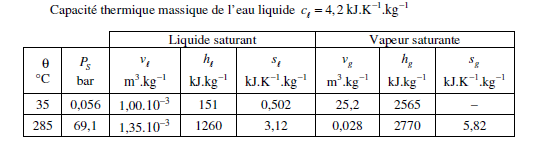
\includegraphics[width=\textwidth]{./Images/mp_s18_ex02.png}

\begin{enumerate}
	\item Représenter avec son sens le cycle décrit par l'eau dans le diagramme de Clapeyron $(P, v)$ et dans le diagramme des frigoristes $(\ln P, h)$. Qualifier chacune des cinq transformations par un ou plusieurs des qualificatifs suivants : isochore, isentropique, isobare, isotherme, adiabatique.
	\item Donner la valeur numérique des enthalpies massiques $h_A$, $h_C$, $h_D$ puis déterminer les entropies massiques $s_A$, $s_B$, $s_C$, $s_D$ et $s_E$.
	\item Calculer le titre en vapeur $x_E$ et l'enthalpie massique $h_E$.
	\item Calculer le transfert thermique massique reçu par le fluide dans le condenseur.
	\item On étudie la compression dans la pompe. On considère que le travail fourni par la pompe est négligeable devant les autres échanges énergétiques du cycle. En déduire $h_A = h_B$.
	\item Calculer le transfert thermique massique $q_{BD}$ fourni par le générateur de vapeur.
	\item Calculer le travail massique utile $w_u$ reçu par l'eau au cours du cycle.
	\item Sachant que la centrale développe une puissance de $\SI{900}{MW}$, calculer le débit massique du fluide dans le circuit.
	\item Quel est le rendement thermodynamique du cycle ? Le comparer au rendement de Carnot et commenter.
\end{enumerate}

\e{Réponses :}
\begin{enumerate}
	\item -
	\item hA = 151, hC = 1260, hD = 2770, sA = 0.502 = sB, sC = 3.12, sD = 5.82 = sE.
	\item xE = 0.68, hE = 1790.
	\item qEA = -1640
	\item qBD = 2620
	\item wu = -981
	\item Dm = 917 kg/s
	\item $\eta$=0.37 et carnot = 0.45	
\end{enumerate}

\subsection{Exercice 3 : Installation frigorifique}

On modélise le comportement thermodynamique du fluide dans une machine frigorifique à fluide diphasé par la succession de transformations suivantes :

\begin{itemize}
	\item Compression adiabatique réversible en phase gazeuse du point d'équilibre A au point d'équilibre B. En A, le fluide est à l'état de vapeur saturante.
	\item Refroidissement isobare de la vapeur de B en C. En C, le fluide est à l'état de vapeur saturante.
	\item Liquéfaction isobare et totale du fluide du point d'équilibre C au point d'équilibre D. Au point D, le fluide est à l'état de liquide saturant.
	\item Détente adiabatique irréversible du fluide que l'on peut ici modéliser par une détente isenthalpique entre D et E.
	\item Vaporisation totale isobare du fluide de E vers A.
\end{itemize}

On donne les enthalpies massiques du fluide aux points $A$, $B$ et $D$ : $$h_A = \SI{1167}{kJ\per\kilogram},~h_B = \SI{1355}{kJ\per\kilogram},~h_D = \SI{30}{kJ\per\kilogram}$$

\begin{enumerate}
	\item Représenter le cycle sur un diagramme de Clapeyron et un diagramme des frigoristes. Calculer les transferts thermiques $q_c$ et $q_f$ reçus par le fluide.
	\item Estimer le coefficient d'efficacité de la machine frigorifique.
	\item La phase gazeuse, de capacité thermique massique à pression constante $c_P$, peut être assimilée à un gaz parfait. Exprimer littéralement l'enthalpie massique de vaporisation $l_v(T_C)$ du fluide à la température au point C $T_C$ en fonction de $T_C$, $c_P$, $T_B$.
	\item Calculer numériquement le titre massique en vapeur $x_E$ sachant que l'enthalpie de vaporisation du fluide à la température $T_A$ est $l_v(T_A) = \SI{1293}{kJ\per\kilogram}$.
	\item On utilise cette installation frigorifique pour maintenir constante la température d'une chambre froide à laquelle il faut enlever $\SI{5000}{kJ}$ par heure. Calculer le débit massique $D_m$ du fluide frigorifique.
\end{enumerate}

\e{Réponses :}
\begin{enumerate}
	\item qc = -1325, qf = 1137
	\item eta = 6. Cela signifie qu'avec 1 J électrique fourni la machine peut ôter 6 J aux aliments à réfrigérer et donc évacuer 7 J dans l'air de la cuisine.
	\item hD-hB = -lv + cp(Tc-Tb)
	\item x = 0.12
	\item 1.22 g/s
\end{enumerate}




\backmatter
% bibliography, glossary and index would go here.

\end{document}